\chapter[Evaluation]{Evaluation}

This chapter provides an evaluation of the NVM Middleware. Firstly, we describe the experimental setup utilized for our evaluations. Next, we assess the performance advantages derived from the concurrency control mechanism integrated into the NVM Middleware. Finally, we evaluate the effectiveness of our reinforcement learning model and Q-Learning algorithm. Specifically, we train an agent and subsequently assess its capacity to adhere to predefined service level agreements amidst dynamic workload variations.
\section{Experimental Setup}

\subsection{Platform}

\begin{table}[ht]
    \centering
    \label{table:platform_specifications}
    \caption{Experimental Platform Specifications}
    \begin{tabular}{|l|l|}
      \hline
      Processor & Intel\,\textsuperscript{\tiny\textregistered} Xeon\,\textsuperscript{\tiny\textregistered} Gold 6252   \\\hline
      Sockets & 2 \\\hline
      Cores per socket & 24  \\\hline
      Threads per core & 2 \\\hline
      Numa nodes & 2 \\\hline
      CPU Frequency & 2.7 GHz (3.7 GHz Turbo frequency) \\\hline
      L1d cache & 1.5 MiB  \\\hline
      L1i cache & 1.5 MiB  \\\hline
      L2 Cache & 48 MiB  \\\hline
      L3 Cache & 71.5 MiB  \\\hline
      DRAM & 16 GB DDR4 DIMM x 6 per socket  \\\hline
      Persistent Memory & 128 GB Optane PMem DIMMs x 6 per socket  \\\hline
      Operating System & Ubuntu 20.04.4 LTS (Focal Fossa)  \\
      \hline
    \end{tabular}
\end{table}

The experimental platform utilized in this study is detailed in Table \ref{table:platform_specifications}. It features an Intel\textsuperscript{\tiny\textregistered} Xeon\textsuperscript{\tiny\textregistered} Gold 6252 processor with 2 sockets, each hosting 24 cores and 2 threads per core, totaling 2 NUMA nodes. Each socket is equipped with three memory channels, housing 16 GB DDR4 DIMMs and 128 GB Optane PMem DIMMs. In aggregate, the system comprises 192 GB of DRAM and 1.5 TB of persistent memory. To mitigate the NUMA effect, one socket is designated for running the NVM Middleware threads, while the other handles the interactive and batch applications, as described in Section 3.4.3.

\subsection{Optane PMem Configuration}
As outlined earlier, this thesis concentrates on exploring the persistent capabilities of Optane PMem. Consequently, Optane PMem is employed in the App Direct Mode throughout our experiments. To facilitate the utilization of persistent memory, we expose it via an xfs filesystem configured in dax mode, thereby bypassing the page cache. Additionally, we enhance memory management and performance by configuring the persistent memory with huge pages (2MiB) \cite{Speeding28:online}. Lastly, we deploy a PMEMKV database with a capacity of 600GB, configured with its persistent concurrent engine.

\subsection{Workload Generators}

We deploy the interactive and batch applications outlined in Section 3.4.3 utilizing two distinct workload generators.

\subsubsection{Yahoo! Cloud Serving Benchmark (YCSB)}

YCSB \cite{GitHubba9:online} is a multi-threaded benchmark specifically tailored for assessing cloud-based databases and storage systems. Utilizing YCSB, we emulate interactive applications by generating small byte requests. To vary the workload characteristics, we modify parameters such as the read-to-write ratio, request distribution, and client threads. Leveraging the C++ version of YCSB, we extend its functionality to facilitate API calls to the NVM Middleware.

\subsubsection{Serverless Trace Replay}

We develop the Serverless Trace Replay tool in-house to replicate workloads typically encountered in real-world serverless environments. This tool operates by reading a file containing workload traces and executing them accordingly. To simulate multiple serverless functions, the tool spawns multiple threads to issue requests concurrently.

For emulating an interactive application, we utilize traces collected from Azure Functions, sourced from a dataset available in \cite{GitHubAz35:online}. This dataset (described in more detail in \cite{romero2021faat}) offers a comprehensive log of Azure Function blob accesses over HTTPS recorded between November and December 2020. Specifically, our experiments utilize requests recorded on December 6, 2020, with a specific emphasis on those involving small data access sizes (less than 1 KB), which typically signify interactive application behavior.

For modeling a batch application, we collect traces from Wukong, a serverless parallel computing framework \cite{carver2020wukong}. The traces are acquired by executing a Single Value Decomposition job for a $128kx128k$ matrix on Wukong and capturing the resulting I/O requests generated by the framework. This dataset offers a precise representation of throughput-oriented serverless data-analytics applications, characterized by significant parallelism and substantial data access sizes spanning from 4KB to 200MB.

% To further amplify the concurrency of requests directed to the NVM Middleware, we accelerated the pace of the traces by a factor of 5 compared to their original timing.

\section{Efficiency of the Workload-Aware Concurrency Control Mechanism}

We evaluate the effectiveness of the workload-aware concurrency control mechanism embedded within the NVM Middleware compared to a baseline scenario devoid of concurrency control. In the baseline setting, concurrency control is inactive, permitting a maximum of 200 concurrent data accesses on Optane PMem. This assessment involves deactivating the reinforcement learning agent and system monitoring, with a primary focus on the 99th percentile latency and throughput observed by client applications.

Six experiments are conducted, running concurrently YCSB and the Serverless Trace Replay simulating SVD traces. Each YCSB experiment varies parameters such as data access size (64B, 128B), read-to-write ratio (50-50, 100-0), and data request distribution (zipfian, uniform), while the Serverless Trace Replay maintains consistent settings across experiments. Both applications are executed with 100 client threads.

In each experiment, the baseline scenario is executed without concurrency control, followed by 42 additional tests exploring various combinations of interactive and batch threads within the NVM Middleware. Each run maintains a fixed combination of interactive ($I$) and batch ($B$) threads. Subsequently, the 99th percentile latency observed by YCSB requests and the overall throughput reported by the Serverless Trace Replay are recorded. The results are depicted in Figures \ref{fig:50_50_middleware_eval}, \ref{fig:100_0_middleware_eval}, and \ref{fig:uniform_50_50_middleware_eval}.

Our observations indicate substantial benefits from the concurrency control implemented by the NVM Middleware across most scenarios. Relative to the baseline, the NVM Middleware demonstrates potential enhancements,  including up to a $435x$ decrease in the tail 99th percentile latency and an $8x$ increase in throughput.. Notably, certain thread combinations achieve sub-millisecond access latencies with a more predictable behavior, significantly improving application performance. However, improper thread configuration within the NVM Middleware, either insufficient or excessive, results in performance degradation exceeding that of the baseline. This emphasizes the criticality of meticulously selecting the optimal thread combination, as an incorrect choice may yield similar or inferior results compared to operating without concurrency control.

A key query arising from these findings concerns determining the optimal thread combination. We observe that prioritizing interactive threads yields sub-millisecond access latencies but compromises peak throughput. Conversely, increasing batch threads to enhance throughput metrics leads to higher access latencies. Addressing this dilemma entails selecting a combination of interactive and batch threads that satisfies both latency and throughput SLA metrics, a topic elaborated upon in the subsequent section.

\begin{figure}
  \centering
  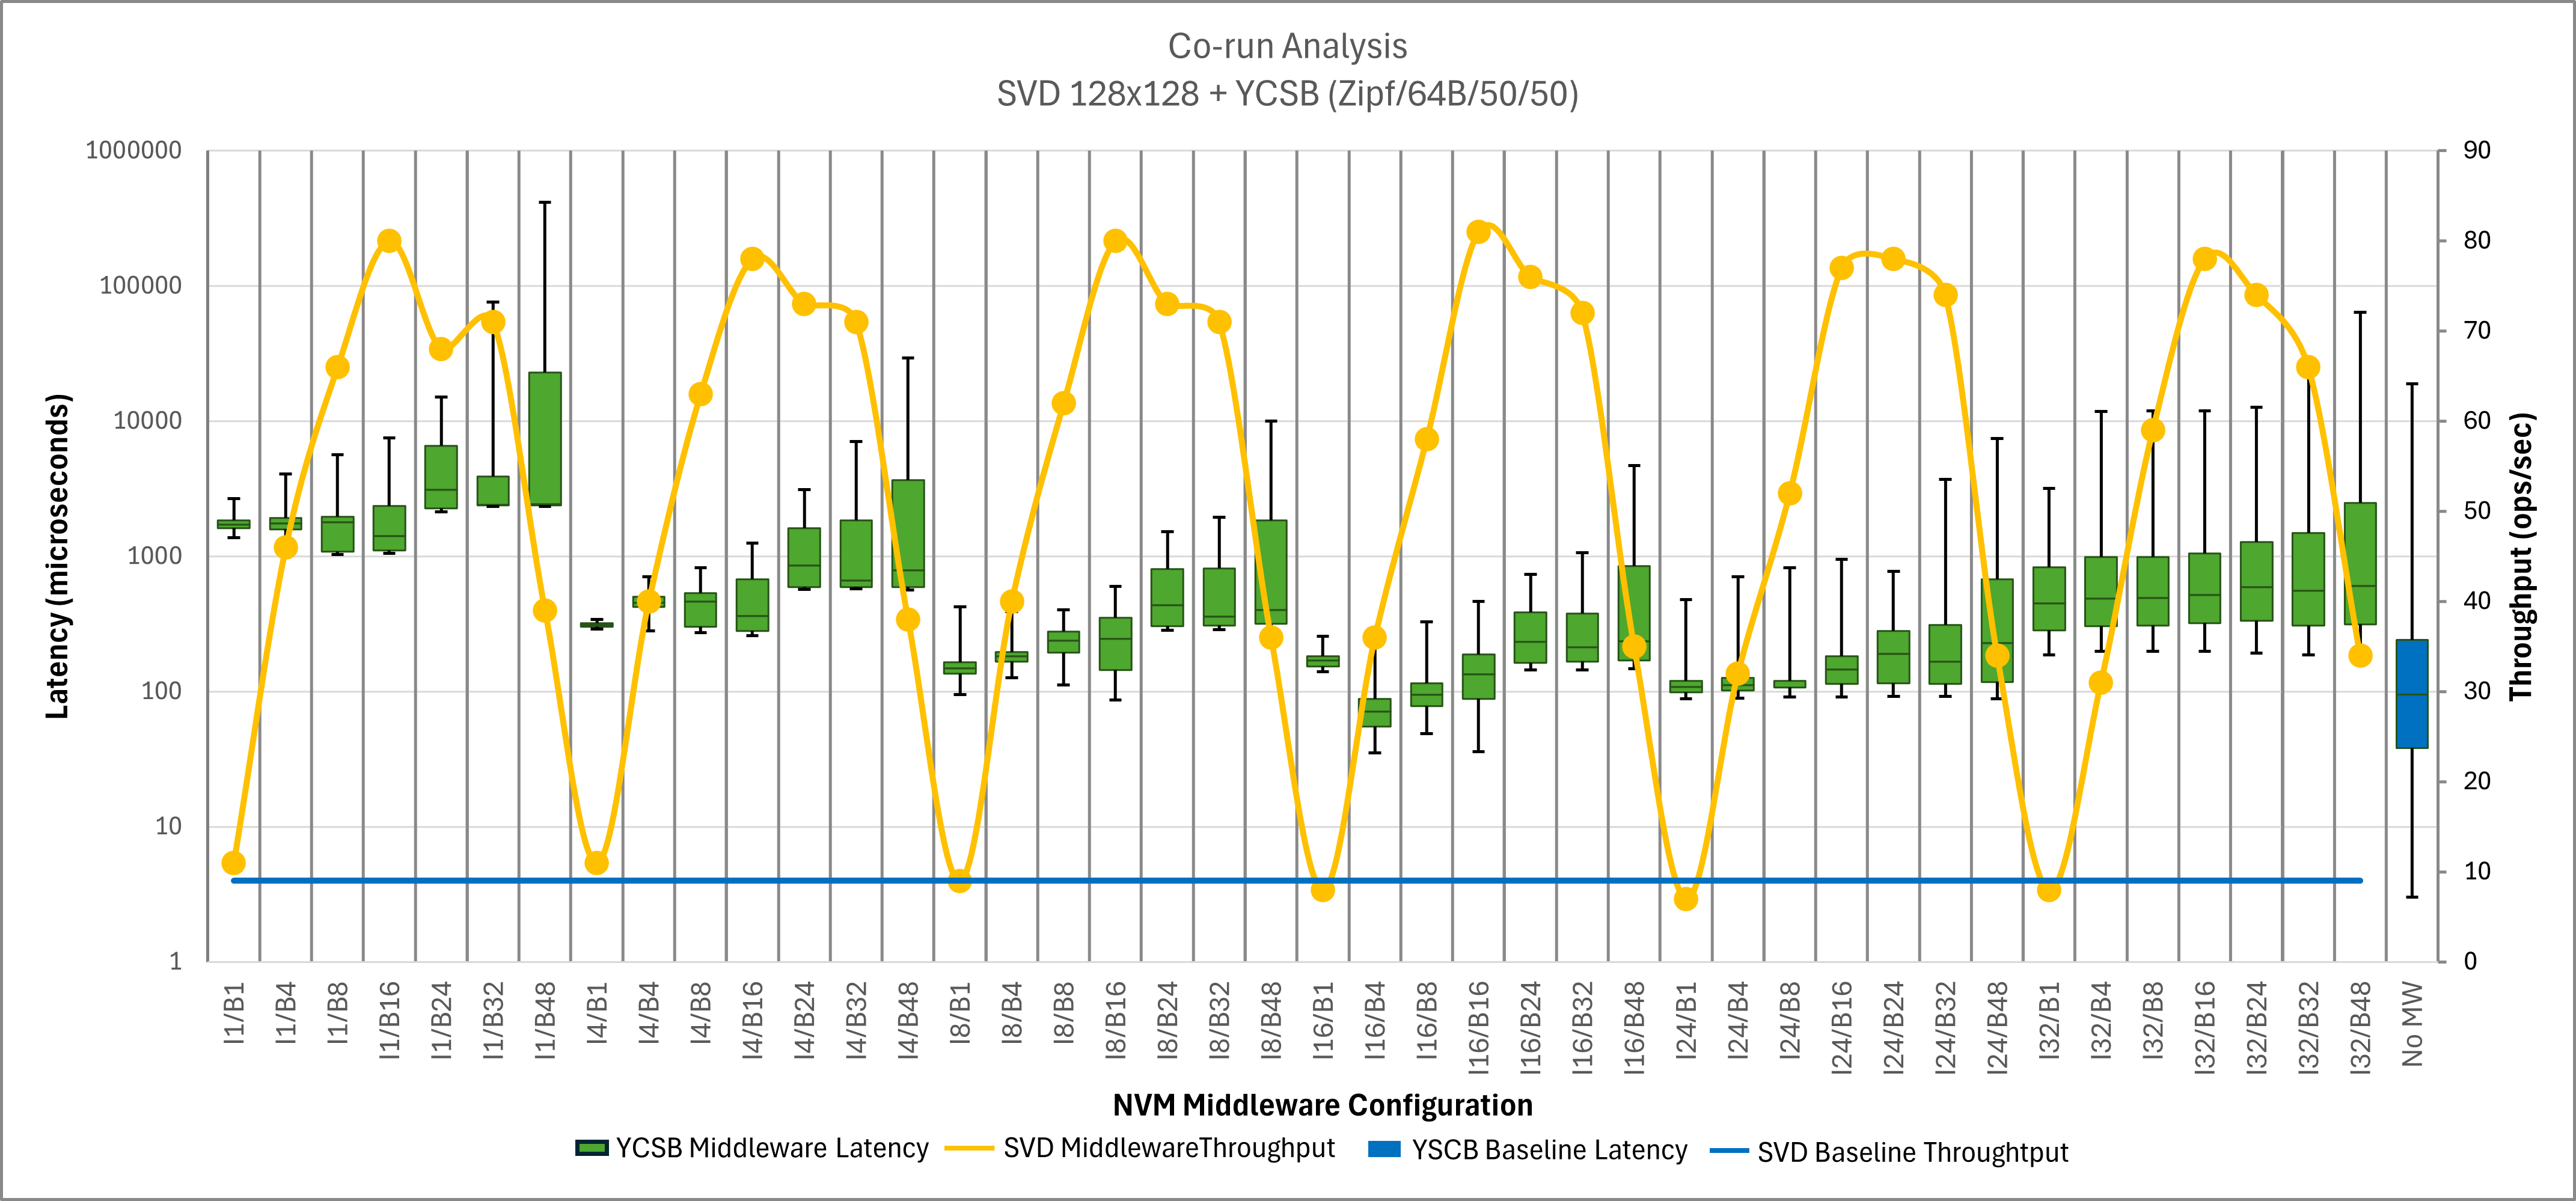
\includegraphics[width=0.8\textwidth,height=\textheight,keepaspectratio,angle=0]{images/64b_50_50_middleware_eval.png}
  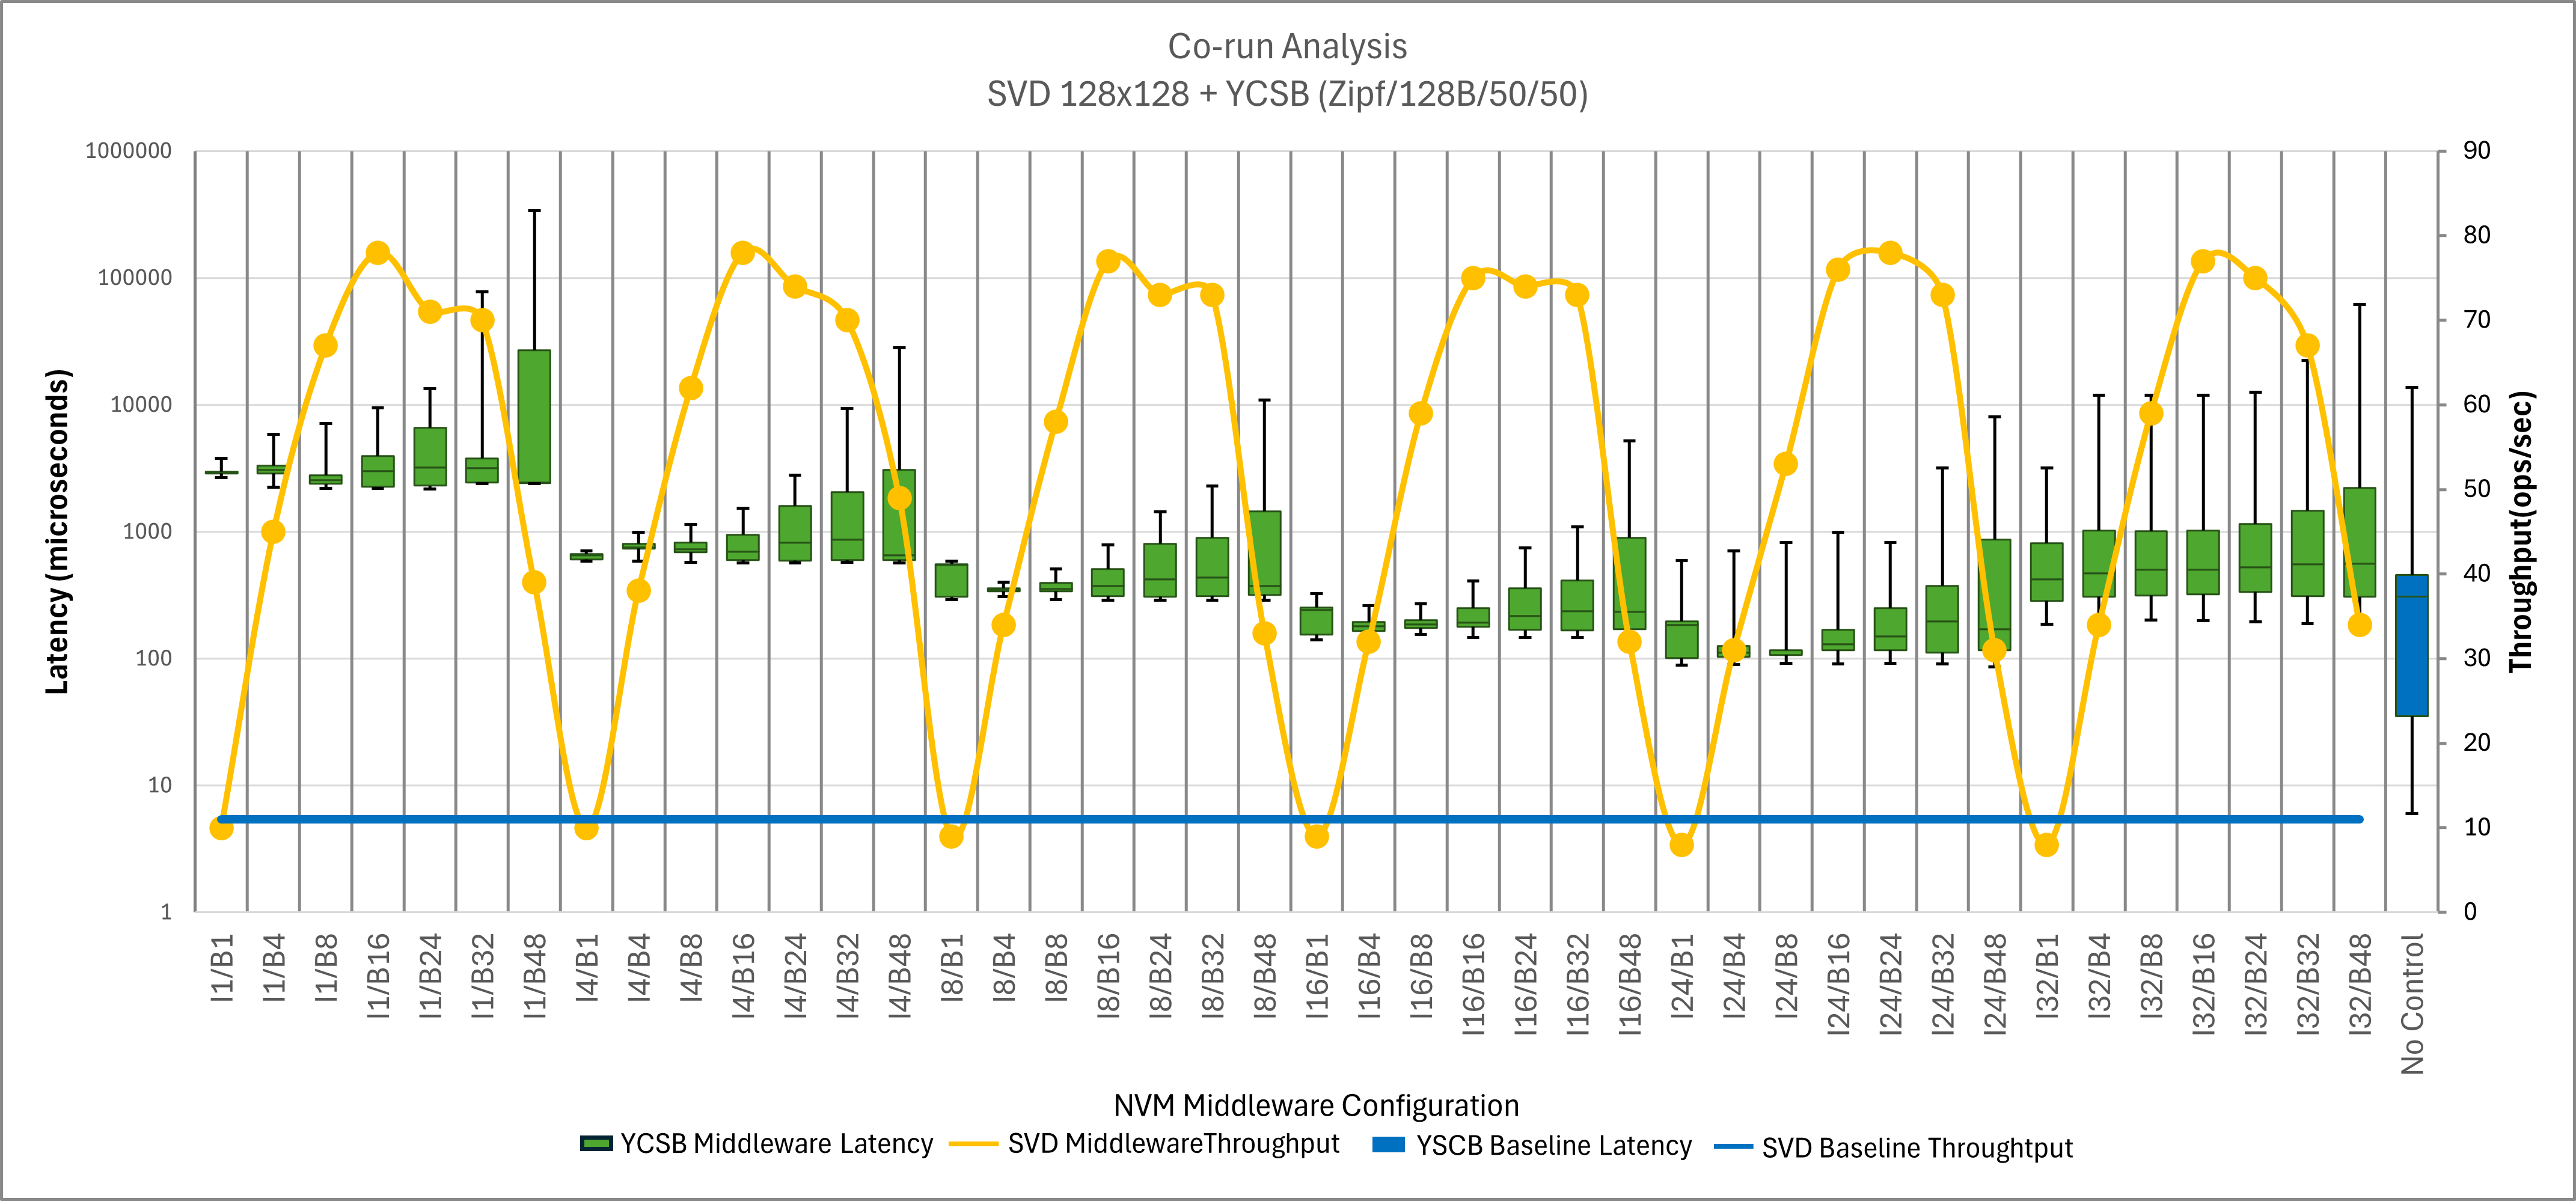
\includegraphics[width=0.8\textwidth,height=\textheight,keepaspectratio,angle=0]{images/128b_50_50_middleware_eval.png}
  % \caption[Evaluation of NVM Middleware: Benchmark A]{Evaluation of the NVM Middleware's concurrency control mechanism when co-running a batch workload and a interactive workload with Zipfian request distribution and even distribution of read and write requests. The interactive workload is generated by YCSB, and two runs are performed configuring YCSB with 64B and 128B data access sizes. Both applications utilize 100 client threads to send requests to the NVM Middleware. The throughput (yellow line) and 99th percentile latency (green box plot) of each application are observed and compared against a baseline with no concurrency control (blue line and box plot).}
  \caption[Evaluation of NVM Middleware: Benchmark A]{Evaluation of the NVM Middleware's concurrency control mechanism when co-running SVD I/O traces (batch) and a YCSB workload (interactive) configured with zipfian request distribution and an even distribution of read and write requests. Two runs are performed configuring YCSB with 64B and 128B data access sizes. Both applications utilize 100 client threads to send requests to the NVM Middleware. The illustration presents statistics on throughput (yellow line) and 99th percentile latency (green box plot) obtained under different configurations of the NVM Middleware, denoted as $I/B$ (Interactive threads/Batch threads). These statistics are compared against a baseline scenario with no concurrency control (blue line and blue box plot). The latencies observed by YCSB are depicted as a distribution, ranging from the minimum to the maximum observed, along with quartiles and median values.}
  \label{fig:50_50_middleware_eval}
\end{figure}

\begin{figure}
  \centering
  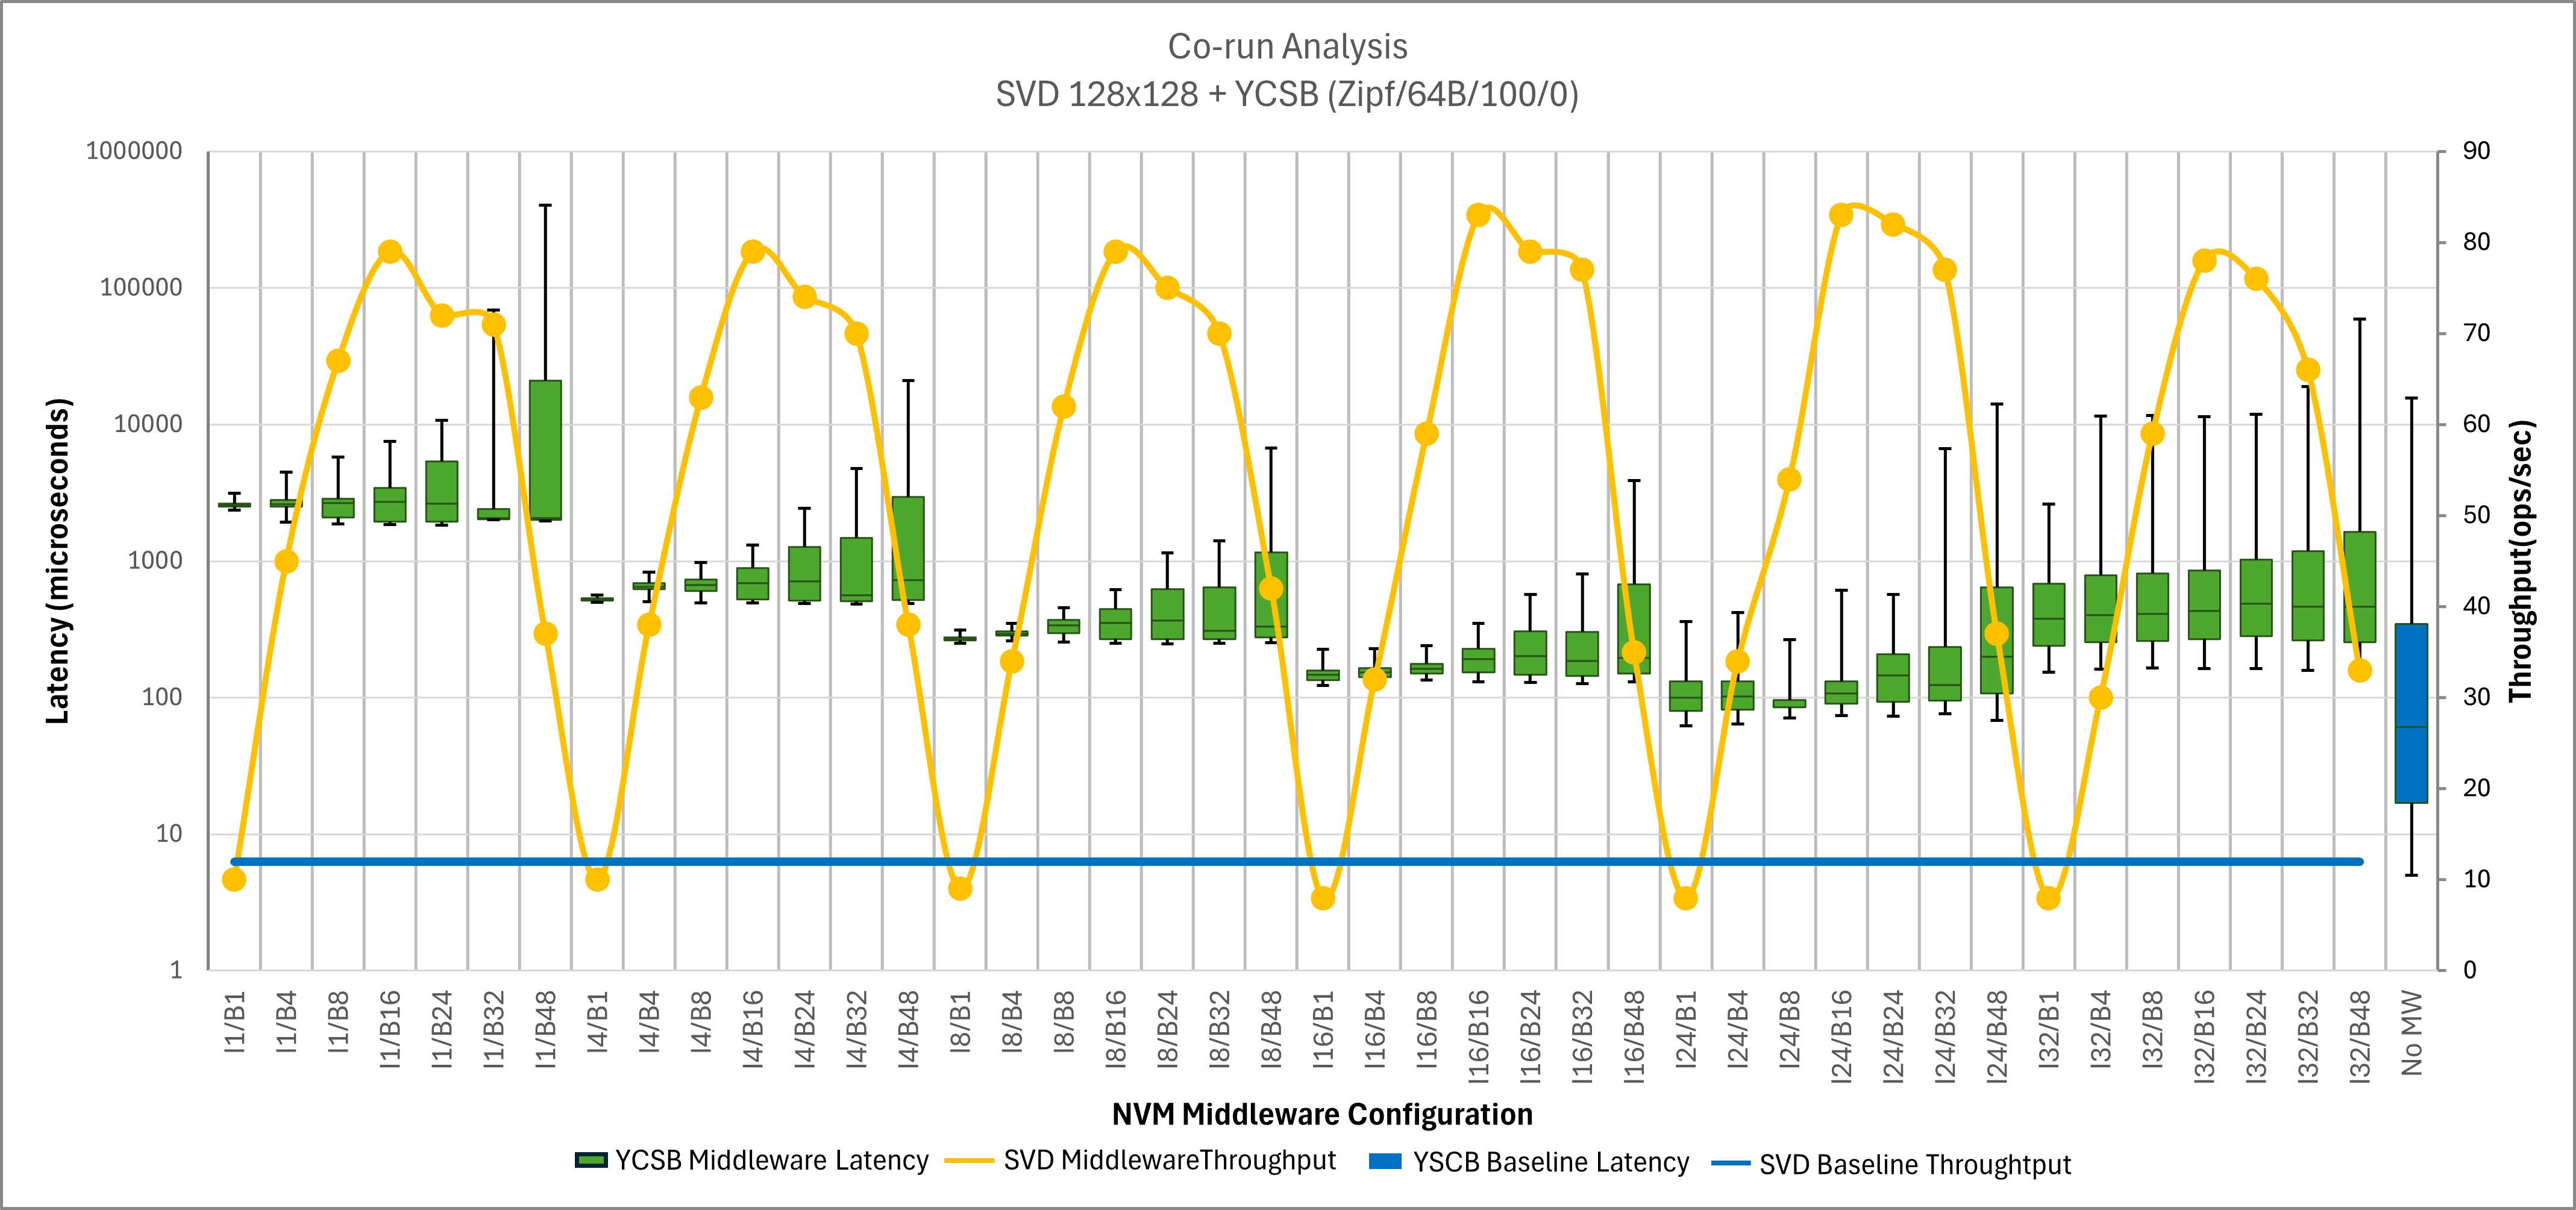
\includegraphics[width=0.8\textwidth,height=\textheight,keepaspectratio,angle=0]{images/64b_100_0_middleware_eval.png}
  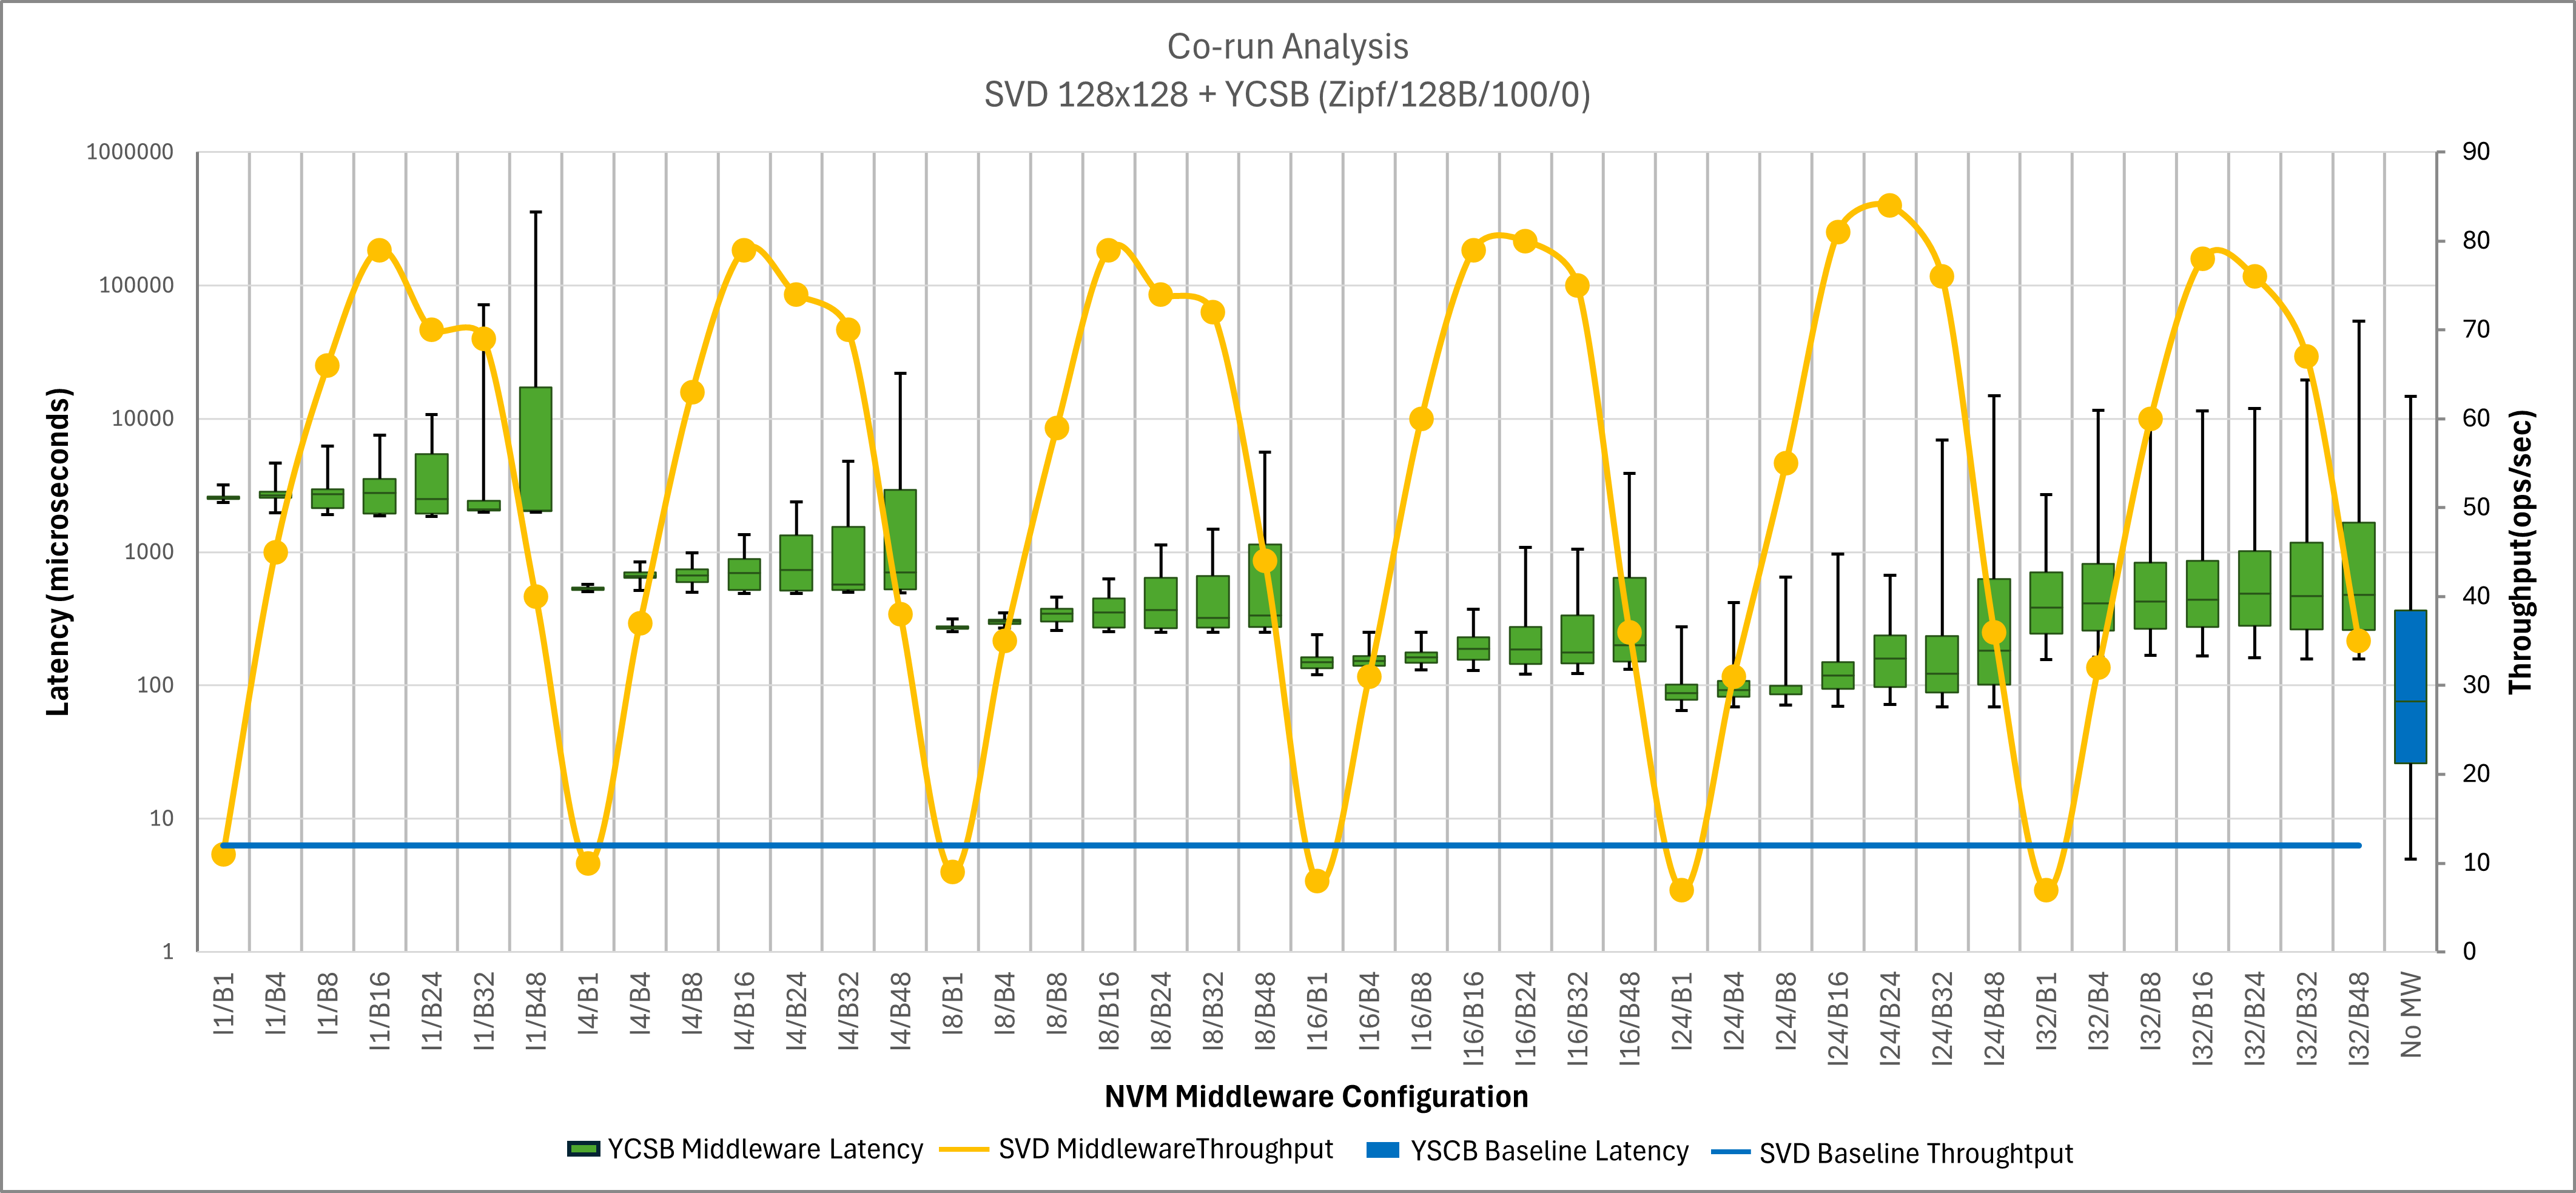
\includegraphics[width=0.8\textwidth,height=\textheight,keepaspectratio,angle=0]{images/128b_100_0_middleware_eval.png}
  % \caption[Evaluation of NVM Middleware: Benchmark B]{Evaluation of the NVM Middleware's concurrency control mechanism when co-running a batch workload and a pure read interactive workload with zipfian request distribution. The interactive workload is generated by YCSB, and two runs are performed configuring YCSB with 64B and 128B data access sizes. Both applications utilize 100 client threads to send requests to the NVM Middleware. The throughput (yellow line) and 99th percentile latency (green box plot) of each application are observed and compared against a baseline with no concurrency control (blue line and box plot).}
  \caption[Evaluation of NVM Middleware: Benchmark B]{Evaluation of the NVM Middleware's concurrency control mechanism when co-running SVD I/O traces and a pure read YCSB workload with Zipfian request distribution. Two runs are performed configuring YCSB with 64B and 128B data access sizes. Both applications utilize 100 client threads to send requests to the NVM Middleware.  The illustration presents statistics on throughput (yellow line) and 99th percentile latency (green box plot) obtained under different configurations of the NVM Middleware, denoted as $I/B$ (Interactive threads/Batch threads). These statistics are compared against a baseline scenario with no concurrency control (blue line and blue box plot). The latencies observed by YCSB are depicted as a distribution, ranging from the minimum to the maximum observed, along with quartiles and median values.}
  \label{fig:100_0_middleware_eval}
\end{figure}

\begin{figure}
  \centering
  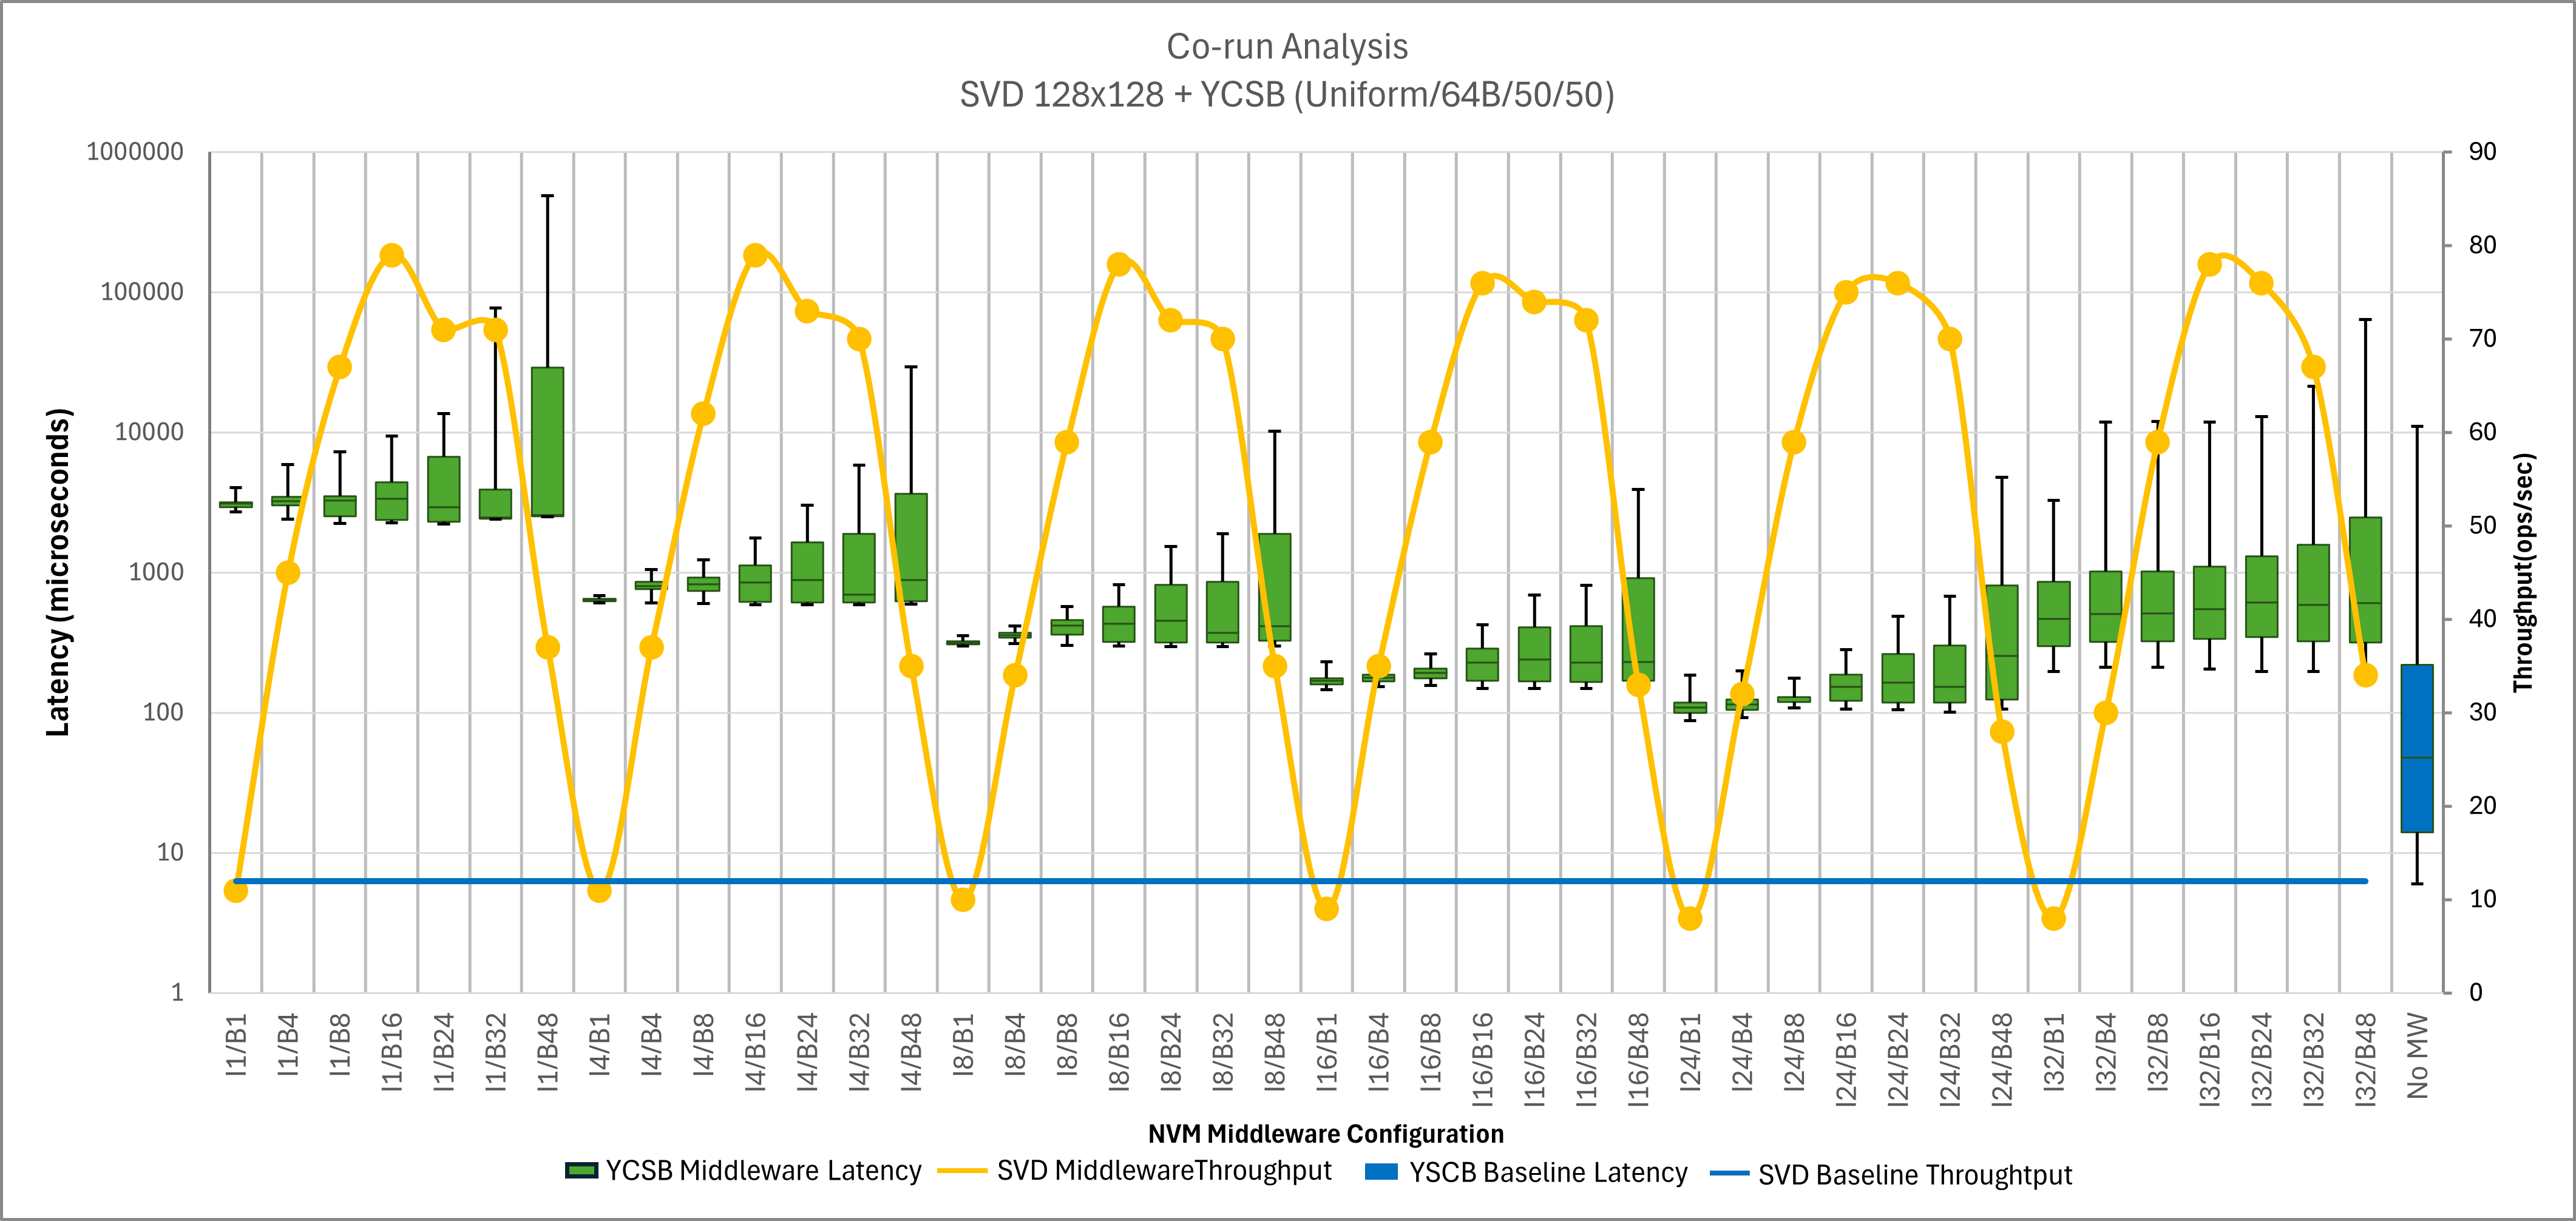
\includegraphics[width=0.8\textwidth,height=\textheight,keepaspectratio,angle=0]{images/64b_uniform_50_50_middleware_eval.png}
  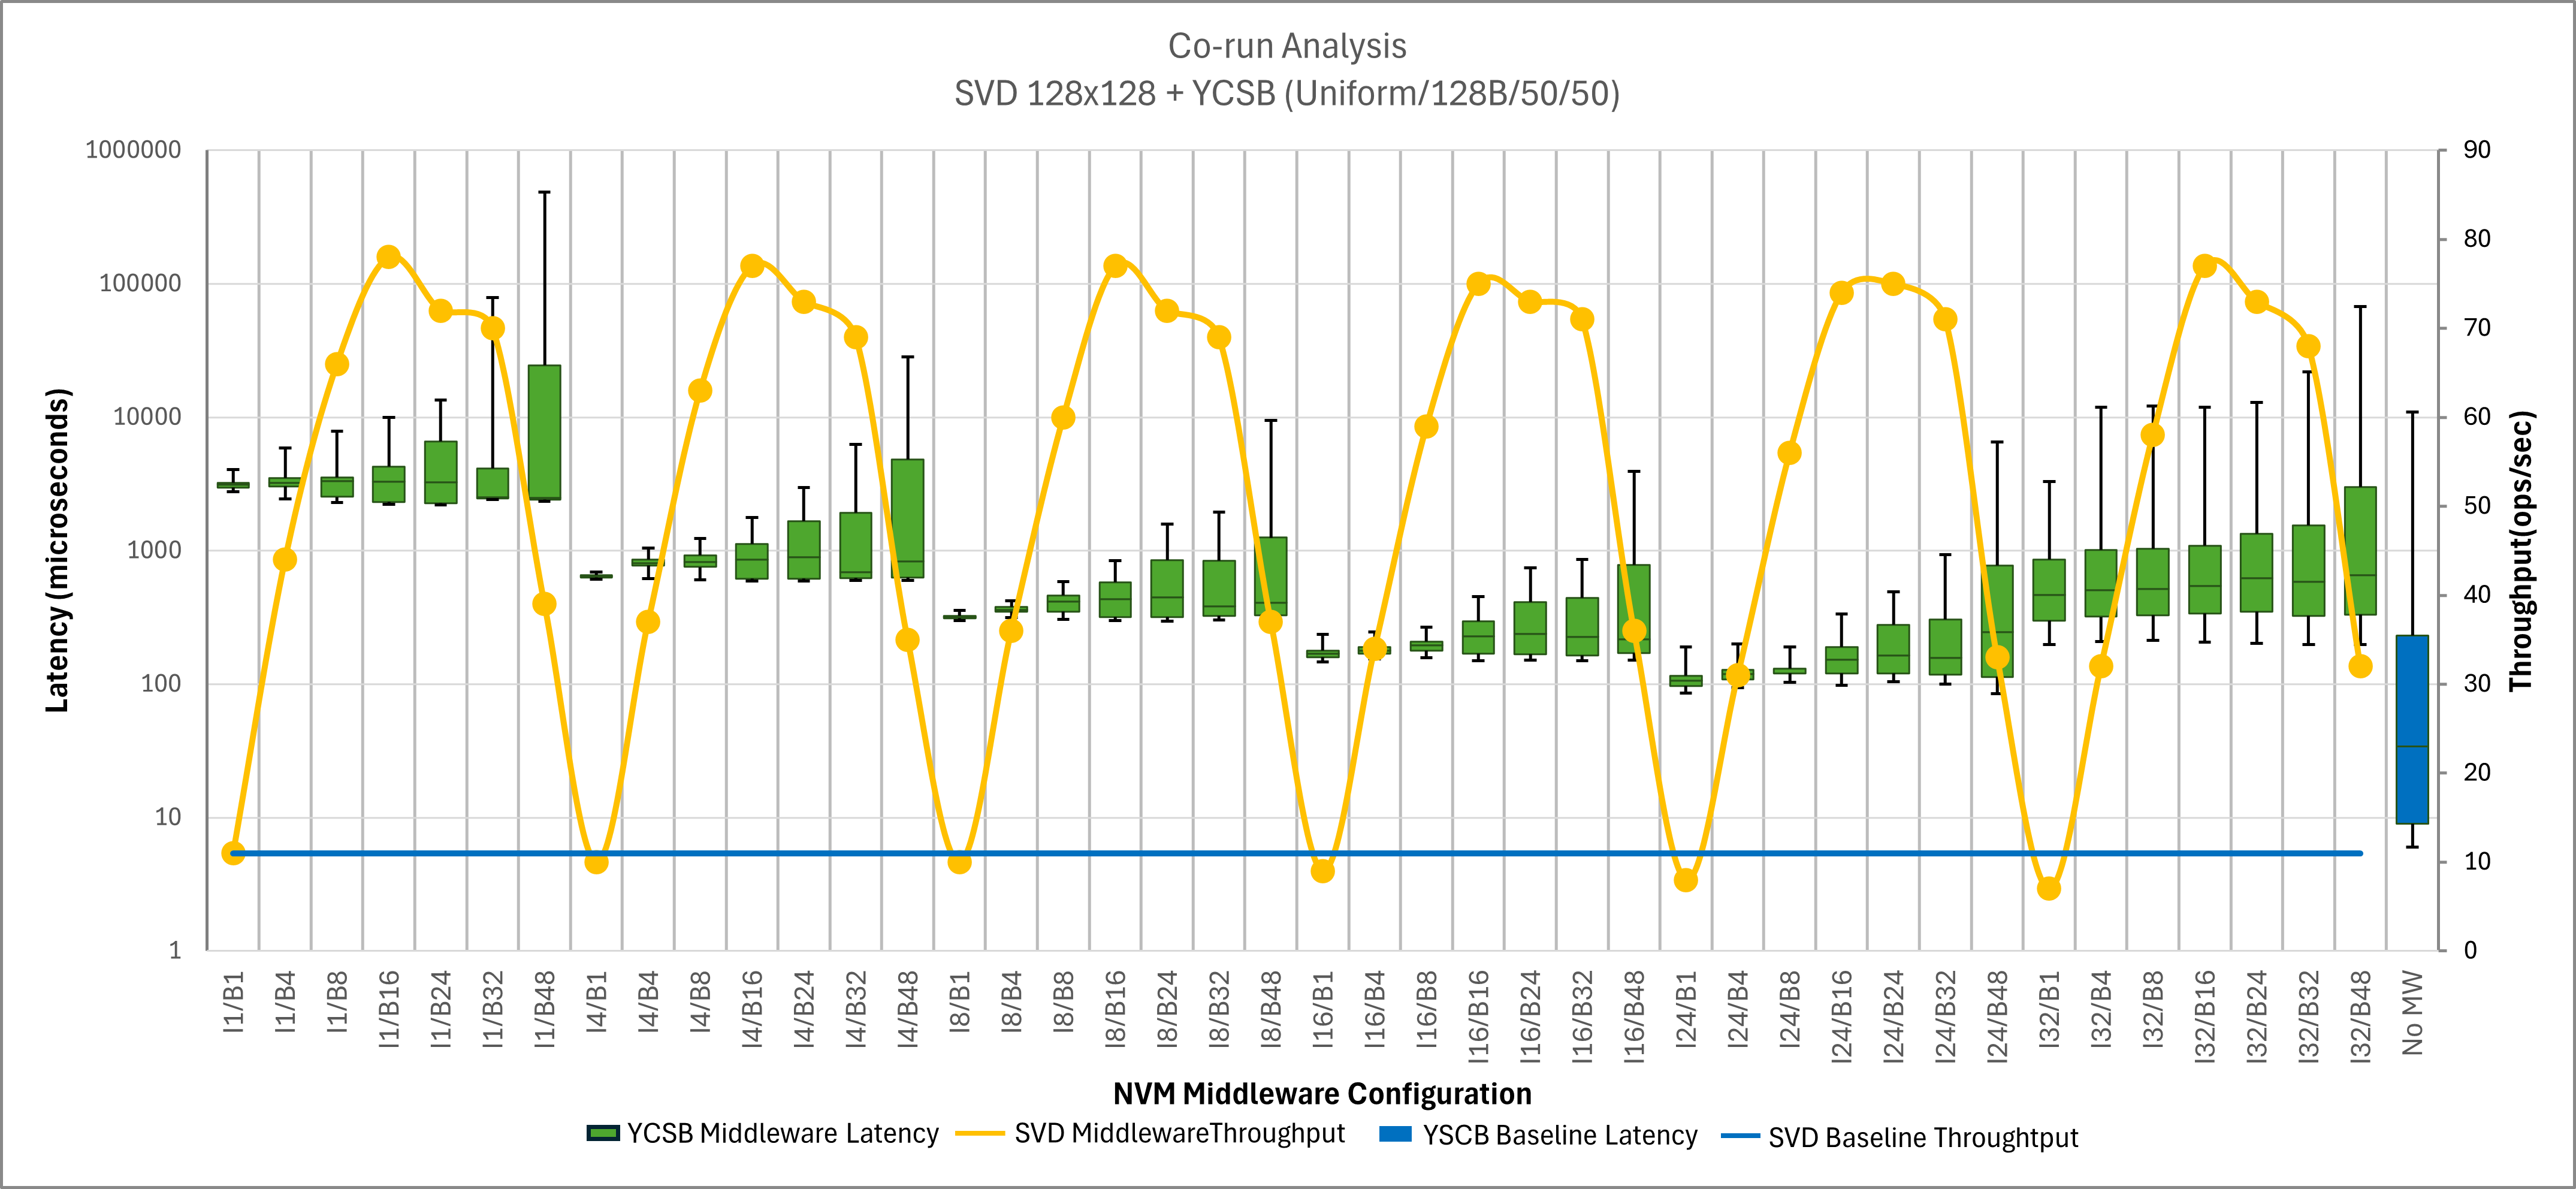
\includegraphics[width=0.8\textwidth,height=\textheight,keepaspectratio,angle=0]{images/128b_uniform_50_50_middleware_eval.png}
  % \caption{Evaluation C}
  % \caption[Evaluation of NVM Middleware: Benchmark C]{Evaluation of the NVM Middleware's concurrency control mechanism when co-running a batch workload and a YCSB workload configured with uniform request distribution and even distribution of read and write requests. The interactive workload is generated by YCSB, and two runs are performed configuring YCSB with 64B and 128B data access sizes. Both applications utilize 100 client threads to send requests to the NVM Middleware. The throughput (yellow line) of the SVD application and 99th percentile latency (green box plot) of YCSB are observed and compared against a baseline with no concurrency control (blue line and box plot).}
  \caption[Evaluation of NVM Middleware: Benchmark C]{Evaluation of the NVM Middleware's concurrency control mechanism when co-running SVD I/O traces and a YCSB workload configured with uniform request distribution and an even distribution of read and write requests. Two runs are performed configuring YCSB with 64B and 128B data access sizes. Both applications utilize 100 client threads to send requests to the NVM Middleware.  The illustration presents statistics on throughput (yellow line) and 99th percentile latency (green box plot) obtained under different configurations of the NVM Middleware, denoted as $I/B$ (Interactive threads/Batch threads). These statistics are compared against a baseline scenario with no concurrency control (blue line and blue box plot). The latencies observed by YCSB are depicted as a distribution, ranging from the minimum to the maximum observed, along with quartiles and median values.}
  \label{fig:uniform_50_50_middleware_eval}
\end{figure}

\section{Meeting SLA performance using Reinforcement Learning}

We present an evaluation of RL-driven policies aimed at balancing the number of interactive and batch threads to meet latency and throughput SLAs within the NVM Middleware. This experiment assesses the NVM Middleware's ability to achieve predefined SLA objectives amidst varying workloads. To this end, we construct four distinct phases, each comprising a interactive and batch application executed concurrently in the environment. Utilizing the Q-Learning algorithm (outlined in Algorithm \ref{algo:q_learning_mw}), we train the RL agent to determine the optimal combination of interactive and batch threads that maximizes performance while meeting predefined latency and throughput SLA objectives for each phase. We then evaluate the agent's ability to predict and adapt to workload changes in an unknown environment where phases are randomly alternated.

\subsection*{Workload Phases}

To evaluate the learning capabilities of the RL agent in adapting thread combinations for optimal performance and meeting predefined SLA metrics, we design four distinct phases. Leveraging I/O traces collected from Azure Functions and Wukong, we construct interactive and batch workloads by adjusting parameters such as data access size, read-to-write ratio, and client threads for each application. We intensify the workload by accelerating the pace of the traces and loop the execution to ensure sufficient simulation steps.

The phases are structured as follows:

\textbf{Phase 1:} We utilize 2039 requests from Azure Function blob access traces captured on December 6, 2020, between 8:20 PM and 8:22 PM. These requests are primarily reads, with a read-to-write ratio of 80-20 and data access sizes ranging between 30B and 50B. For the batch workload, we employ a subset of SVD traces comprising 3847 requests, maintaining a 50-50 read-to-write ratio and a fixed data access size of 800KB. Both applications are configured with 200 client threads for concurrent request handling.

\textbf{Phase 2:} The interactive workload remains unchanged from Phase 1, while the number of client threads is reduced to 150. Similarly, the batch workload maintains its configuration but with an increased number of concurrent client threads set to 320.

\textbf{Phase 3:} The interactive workload is consistent with Phase 1, but with an escalation in client threads to 400. For the batch workload, we modify the SVD traces to employ a fixed data access size of 4k and transition to a read-only workload. Concurrently, we assign 200 client threads for the batch workload.

\textbf{Phase 4:} Drawing from Azure Function blob access traces, we incorporate 7814 requests occurring on December 6, 2020, between 1:21 PM and 1:27 PM for the interactive workload. These requests are predominantly writes, with a read-to-write ratio of 10-90 and larger data access sizes averaging around 500B. The batch workload configuration remains consistent with Phase 3. Each application is allocated 200 client threads for concurrent request processing.

\subsection*{Training the RL Agent}

We commence the learning process by conducting model selection and hyperparameter tuning on the nine regression models employed by the RL agent (refer to Table \ref{table:hyperparameter_tuning} for tuning options). This entails generating a dataset of transitions in the environment by executing a non-optimal random agent on the environment for 150 episodes of each workload. Subsequently, we utilize these transitions to select the appropriate model and tune hyperparameters for each action. The resulting regression models are summarized in Table \ref{table:per_model_parameters}.

With the tuned regression models, we proceed to execute the Q-learning algorithm for each workload using the parameters detailed in Table \ref{table:rl_training_parameters}. To address the exploration-exploitation dilemma, we initialize the epsilon value to 1 and decay it after each episode. This strategy facilitates comprehensive exploration of the state space early in training, followed by exploitation of acquired knowledge. We note that different phases require varying numbers of training episodes to converge to an optimal pattern, likely due to the initial dataset's generation with a non-optimal policy. Initially, we conduct empirical tests (Tables \ref{table:rewards_phase_1} - \ref{table:rewards_phase_4}) by fixing the NVM Middleware threads to manually ascertain the optimal combination. Subsequently, we execute Q-learning and analyze the last three episodes of each phase to determine the convergent combination of threads.

Our observations (Figures \ref{fig:learned_phase_1} - \ref{fig:learned_phase_4}) indicate that the RL agent is capable of learning the optimal combination of interactive and batch threads for each workload. The learned combination of threads matches our empirical results across all workloads. For Workload A, the agent converges to utilizing approximately 10 interactive and batch threads each. Similarly, for Workload B, the agent converges to approximately 10 interactive and batch threads. For Workload C, the agent converges to approximately 7 interactive and 3 batch threads, while for Workload D, it converges to approximately 15 interactive threads and 5 batch threads.

\begin{table}[!htb]
  \centering
  % \caption[RL Regression Models: Hyperparameter Tuning]{List of parameters used for tuning hyperparameters of the polynomial regression models used for function approximation. $Degree$ represents the degree of the polynomial function. $Loss$ represents the loss funciton used by stochastic gradient descent. regularizer represents the penalty to applied to the loss function to shrink the model parameters towards the zero vector. This technique is widely used in regression models to avoid overfitting the data. $Alpha$ represent the strenght to whic the regularization penalty is applied. $learning\_rate$ represents the learning rate schedul of the model. $Max_iter$ represents the maximum number of passes over the training dat}
  \caption[Hyperparameter Tuning Options for Polynomial Regression Models]{Overview of hyperparameters used in the tuning process for polynomial regression models employed in function approximation. The $degree$ parameter denotes the degree of the polynomial function utilized. The $loss$ parameter specifies the loss function employed during stochastic gradient descent. The $penalty$ parameter represents the regularization technique applied to mitigate overfitting. The $alpha$ parameter indicates the strength of the regularization penalty. The $learning\_rate$ parameter determines the scheduling of the model's learning rate. Finally, the $max\_iterations$ parameter sets the maximum number of passes over the training data.}
  \label{table:hyperparameter_tuning}
  % Tabular environment goes AFTER the caption!
  % \begin{adjustbox}{width=1\textwidth}
  \begin{tabular}{|c|c|}
    % after \\: \hline or \cline{col1-col2} \cline{col3-col4} ...
    \hline
    \thead{Parameter} & \thead{Values} \\
    \hline
    degree & 1,2,3 \\\hline
    loss & squared, huber, epsilon\_insensitive \\\hline
    penalty & l1, l2, elasticnet \\\hline
    alpha & 0.1, 0.01, 0.001, 0.0001 \\\hline
    learning rate & constant, optimal, invscaling \\\hline
    max\_iterations & 100, 1000, 10000, 100000 \\
    \hline
  \end{tabular}
  % \caption{Model Selection and Hyper-parameter Tuning parameters categorized by type.}
% \end{adjustbox}
\end{table}

\begin{table}[!htb]
  \centering
  \caption[Resulting Hyperparameters for Polynomial Regression Models]{Hyperparameters of the polynomial regression models after hyperparameter tuning.}
  \label{table:per_model_parameters}
  % Tabular environment goes AFTER the caption!
  \begin{adjustbox}{width=1\textwidth}
  \begin{tabular}{|l|l|}
    % after \\: \hline or \cline{col1-col2} \cline{col3-col4} ...
    \hline
    \thead{Model} & \thead{Parameters} \\
    \hline
    Model\_1 & \makecell[cl] {degree: 2, learning\_rate: 'invscaling', loss: 'squared\_loss', alpha: 0.1, max\_iter: 1000, \\ penalty: elasticnet} \\\hline
      Model\_2 & \makecell[cl] {degree: 2, learning\_rate: 'invscaling', loss: 'squared\_loss', alpha: 0.01, max\_iter: 10000, \\ penalty: l1} \\\hline
      Model\_3 & \makecell[cl] {degree: 2, learning\_rate: 'invscaling', loss: 'squared\_loss', alpha: 0.0001, max\_iter: 100, \\ penalty: elasticnet} \\\hline
      Model\_4 & \makecell[cl] {degree: 2, learning\_rate: 'invscaling', loss: 'squared\_loss', alpha: 0.001, max\_iter: 10000, \\ penalty: l1} \\\hline
        Model\_5 & \makecell[cl] {degree: 2, learning\_rate: 'invscaling', loss: 'squared\_loss', alpha: 0.01, max\_iter: 10000, \\ penalty: elasticnet} \\\hline
    Model\_6 & \makecell[cl] {degree: 2, learning\_rate: 'invscaling', loss: 'squared\_loss', alpha:  0.01, max\_iter: 1000, \\ penalty: elasticnet} \\\hline
    Model\_7 & \makecell[cl] {degree: 2, learning\_rate: 'invscaling', loss: 'squared\_loss', alpha: 0.01, max\_iter: 1000, \\ penalty: elasticnet} \\\hline
    Model\_8 & \makecell[cl] {degree: 2, learning\_rate: 'invscaling', loss: 'squared\_loss', alpha: 0.1, max\_iter: 10000, \\ penalty: l1} \\\hline
    Model\_9 & \makecell[cl] { degree: 2, learning\_rate: 'invscaling', loss: 'squared\_loss', alpha: 0.01, max\_iter: 100, \\ penalty: elasticnet} \\
    \hline
  \end{tabular}
\end{adjustbox}
\end{table}

\begin{table}[!htb]
  \centering
  \caption[Q-Learning Parameters]{Parameters utilized for Q-Learning by the RL agent. The target 99th percentile latency and throughput represent predefined SLAs guiding the reward calculation. The aim is to maintain the observed 99th percentile latency below 250 microseconds while ensuring throughput remains above 250,000 operations per second. The exploration rate ($epsilon$) diminishes gradually between episodes, following a decay rate ($epsilon\_decay$), to strike a balance between exploration and exploitation of knowledge. Furthermores, additional episodes beyond the initially specified count are introduced to enable the agent to reach the optimal policy for phases 1, 3, and 4.}
  \label{table:rl_training_parameters}
  % Tabular environment goes AFTER the caption!
  % \begin{adjustbox}{width=1\textwidth}
  \begin{tabular}{|c|c|}
    % after \\: \hline or \cline{col1-col2} \cline{col3-col4} ...
    \hline
    \thead{Parameter} & \thead{Value} \\
    \hline
    episodes & Phases $1,3,4$: 1,000, Phase $2$: 700 \\\hline
    steps per episode & 200 \\\hline
    gamma & 0.95 \\\hline
    learning rate & 0.7 \\\hline
    epsilon & 0.9 \\\hline
    epsilon\_decay & 0.1 \\\hline
    Target 99th Latency & $\leq$ 250 microseconds \\\hline
    Target throughput & $\geq$ 250,000 operations/second \\
    \hline
  \end{tabular}
% \end{adjustbox}
\end{table}

\begin{table}[!htb]
  \centering
  % \caption{Preliminary Rewards Phase 1}
  \caption[Preliminary Measurements for Phase 1]{Experimental reward analysis conducted on Phase 1 using the NVM Middleware with various fixed combinations of interactive ($I$) and batch ($B$) threads. The table displays statistics on rewards obtained under different configurations, denoted as I5/B5, I10/B10, I15/B15, I15/B5, and I5/B15. The values represent the distribution of rewards, ranging from the minimum to the maximum observed, along with quartiles and median scores. Based on these preliminary findings, the configuration with 10 interactive threads and 10 batch threads appears to yield the most favorable results for Phase 1.}
  \label{table:rewards_phase_1}
  % Tabular environment goes AFTER the caption!
  % \begin{adjustbox}{width=1\textwidth}
  \begin{tabular}{|c|c|c|c|c|c|}
    % after \\: \hline or \cline{col1-col2} \cline{col3-col4} ...
    \hline
    \thead{} & \thead{I5/B5} & \thead{I10/B10} & \thead{I15/B15} & \thead{I15/B5} & \thead{I5/B15}\\
    \hline
    Min & -5,716 & \cellcolor{green}-8,312 & -41,660 & -5,682 & -9,436\\\hline
    Q1 & -1,383 & \cellcolor{green}2.7 & -4,797 & -2,971 & -1\\\hline
    Median & -171 & \cellcolor{green}3.92 & -2 & -1,850 & 0\\\hline
    Q3 & 0 & \cellcolor{green}4.3 & 3 & -1,035 & 1\\\hline
    Max & 1 & \cellcolor{green}5 & 5 & 3 & 2\\
    \hline
  \end{tabular}
% \end{adjustbox}
\end{table}

\begin{table}[!htb]
  \centering
  % \caption{Preliminary Rewards Phase 2}
  \caption[Preliminary Measurements for Phase 2]{Experimental reward analysis conducted on Phase 2 using the NVM Middleware with various fixed combinations of interactive ($I$) and batch ($B$) threads. The table displays statistics on rewards obtained under different configurations, denoted as I5/B5, I10/B10, I15/B15, I15/B5, and I5/B15. The values represent the distribution of rewards, ranging from the minimum to the maximum observed, along with quartiles and median scores. Based on these preliminary findings, the configuration with 10 interactive threads and 10 batch threads appears to yield the most favorable results for Phase 2.}
  \label{table:rewards_phase_2}
  % Tabular environment goes AFTER the caption!
  % \begin{adjustbox}{width=1\textwidth}
  \begin{tabular}{|c|c|c|c|c|c|}
    % after \\: \hline or \cline{col1-col2} \cline{col3-col4} ...
    \hline
    \thead{} & \thead{I5/B5} & \thead{I10/B10} & \thead{I15/B15} & \thead{I15/B5} & \thead{I5/B15}\\
    \hline
    Min & -4,320 & \cellcolor{green}-7,763 & -20,455 & -5,328 & -10,060\\\hline
    Q1 & -463 & \cellcolor{green}-1.9 & -1,169 & -368 & 1\\\hline
    Median & 1.3 & \cellcolor{green}5.2 & 4.2 & 3.1 & 3\\\hline
    Q3 & 1.8 & \cellcolor{green}5.8 & 4.9 & 3.3 & 4\\\hline
    Max & 2.8 & \cellcolor{green}6 & 6 & 3.8 & 6\\
    \hline
  \end{tabular}
% \end{adjustbox}
\end{table}

\begin{table}[!htb]
  \centering
  % \caption{Preliminary Rewards Phase 3}
  \caption[Preliminary Measurements for Phase 3]{Experimental reward analysis conducted on Phase 3 using the NVM Middleware with various fixed combinations of interactive ($I$) and batch ($B$) threads. The table displays statistics on rewards obtained under different configurations, denoted as I5/B5, I7/B3, I7/B7, I10/B10, I15/B15, I15/B5, and I5/B15. The values represent the distribution of rewards, ranging from the minimum to the maximum observed, along with quartiles and median scores. Based on these preliminary findings, the configuration with 7 interactive threads and 3 batch threads appears to yield the most favorable results for Phase 3.}
  \label{table:rewards_phase_3}
  % Tabular environment goes AFTER the caption!
  % \begin{adjustbox}{width=1\textwidth}
  \begin{tabular}{|c|c|c|c|c|c|c|c|}
    % after \\: \hline or \cline{col1-col2} \cline{col3-col4} ...
    \hline
    \thead{} & \thead{I5/B5} & \thead{I7/B3} & \thead{I7/B7} & \thead{I10/B10} & \thead{I15/B15} & \thead{I15/B5} & \thead{I5/B15}\\
    \hline
    Min & -12,490 & \cellcolor{green}-6,582 & -174,852 & -141,354 & -149,647 & -96,900 & -13,211\\\hline
    Q1 & -1,230 & \cellcolor{green}-1,727 & -2,567 & -18,768 & -42,951 & -58,414 & -8,583\\\hline
    Median & -272 & \cellcolor{green}-672 & -4 & -566 & -14,008 & -2,954 & -4,940\\\hline
    Q3 & -5 & \cellcolor{green}-3 & -2 & -1 & -4,607 & 0 & -2,709\\\hline
    Max & -3 & \cellcolor{green}-1 & 0 & 3 & -1 & 4 & -943\\
    \hline
  \end{tabular}
% \end{adjustbox}
\end{table}

\begin{table}[!htb]
  \centering
  % \caption{Preliminary Rewards Phase 4}
  \caption[Preliminary Measurements for Phase 4]{Experimental reward analysis conducted on Phase 4 using the NVM Middleware with various fixed combinations of interactive ($I$) and batch ($B$) threads. The table displays statistics on rewards obtained under different configurations, denoted as I5/B5, I10/B10, I15/B15, and I15/B5. The values represent the distribution of rewards, ranging from the minimum to the maximum observed, along with quartiles and median scores. Based on these preliminary findings, the configuration with 15 interactive threads and 5 batch threads appears to yield the most favorable results for Phase 4.}
  \label{table:rewards_phase_4}
  % Tabular environment goes AFTER the caption!
  % \begin{adjustbox}{width=1\textwidth}
  \begin{tabular}{|c|c|c|c|c|}
    % after \\: \hline or \cline{col1-col2} \cline{col3-col4} ...
    \hline
    \thead{} & \thead{I5/B5} & \thead{I10/B10} & \thead{I15/B15} & \thead{I15/B5}\\
    \hline
    Min & -11,341 & -14,699 & -21,259 & \cellcolor{green}-3,912\\\hline
    Q1 & -153 & -2.5 & -6,908 & \cellcolor{green}-1\\\hline
    Median & -2 & 2.3 & -3,117 & \cellcolor{green}3\\\hline
    Q3 & 0 & 3.7 & -4 & \cellcolor{green}4\\\hline
    Max & 3 & 5 & 3 & \cellcolor{green}5\\
    \hline
  \end{tabular}
% \end{adjustbox}
\end{table}

\begin{figure}[!htb]
  \centering
  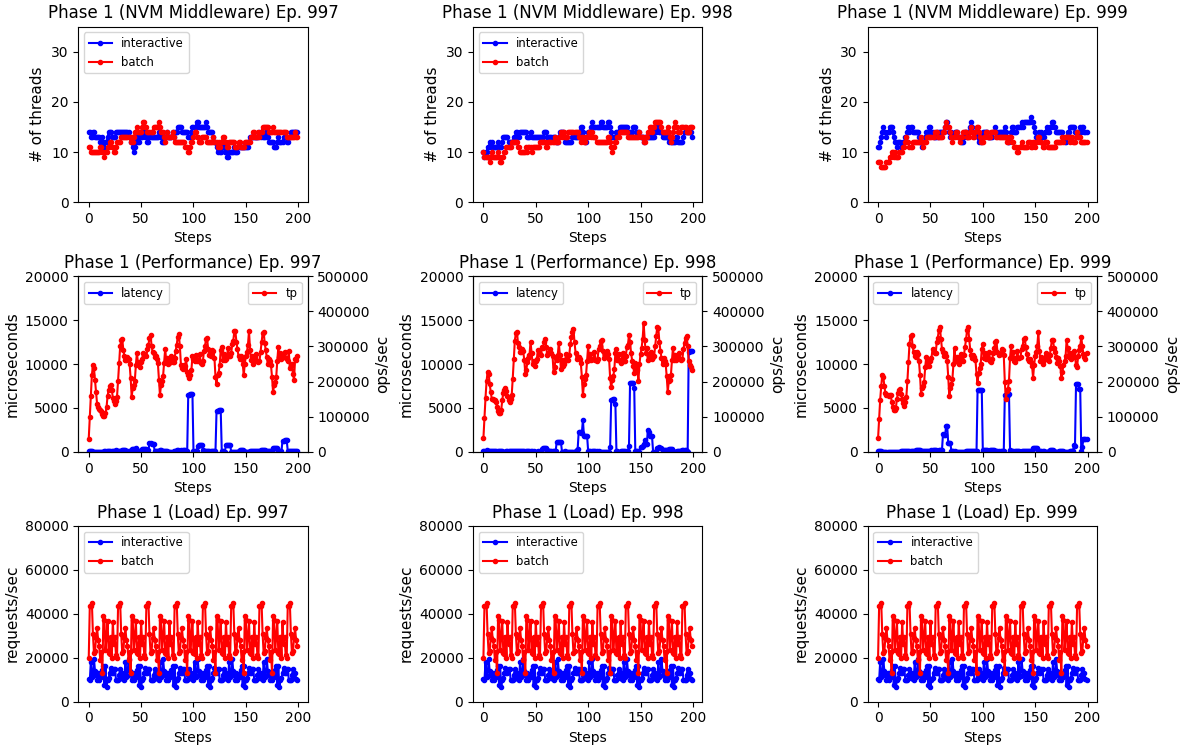
\includegraphics[width=\textwidth,height=\textheight,keepaspectratio,angle=0]{images/rl_training_phase1.png}
  % \caption[Phase 1: Agent's Learned Pattern]{Analysis of the three last episodes of the Q-Learning process performed by the agent when running Phase 1 for 1,000 episodes. On these episodes, the exploration rate is low, indicating that the agent is exploiting its knowledge acquired from previous episodes. The first row demonstrated that the agent configures the NVM Middleware with 10 interactive and 10 batch threads when it starts receiving requests sent from applications configured in Phase 1. This combination of threads matches the preliminary resutls obtained for this phase. Additionally, the second row demonstrates how by configuring the NVM Middleware with the optiomal combination of threads, the agent, most of the steps, keeps the latency low (less than 250 microseconds) and the throughput below 250,000 operations/second.}
  \caption[Learned Pattern of Agent during Phase 1]{Visualization depicting the learned pattern of the agent during Phase 1 of the training process. The analysis focuses on the behavior observed in the final three episodes of the Q-Learning process, which spanned 1,000 episodes. During these episodes, the exploration rate is so low that the agent predominantly exploits its accumulated knowledge. The first row illustrates the agent's configuration of the NVM Middleware with approximately 10 interactive and 10 batch threads, aligning with preliminary results for Phase 1. In the middle row, the throughput and 99th percentile latency reported by the NVM Middleware at each time step are depicted. By employing the optimal combination of threads, the agent consistently maintains low latency (less than 250 microseconds) and a throughput exceeding 250,000 operations/second across most steps. Finally, the bottom row illustrates the operations per second sent to the NVM Middleware by Phase 1.}
  \label{fig:learned_phase_1}
\end{figure}

\begin{figure}[!htb]
  \centering
  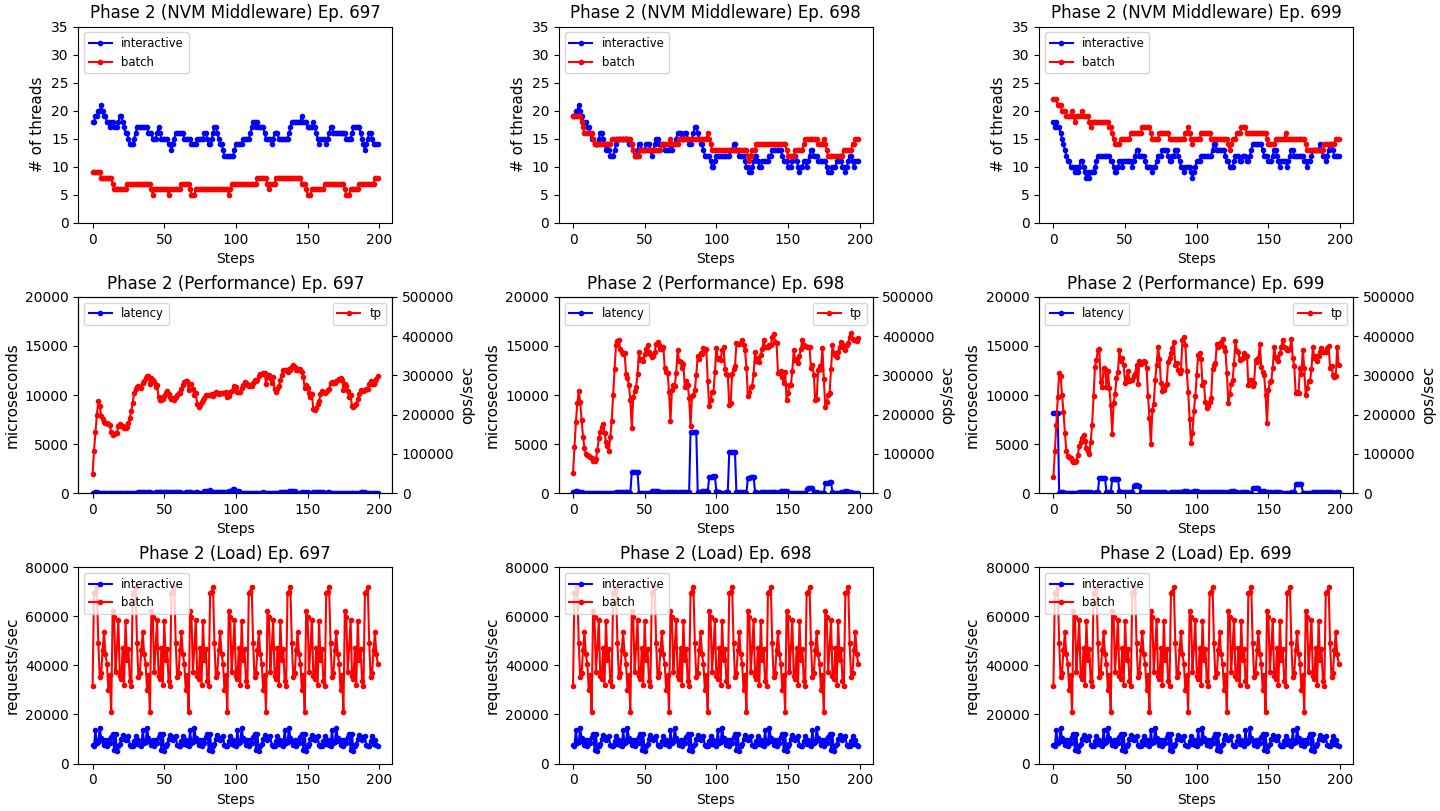
\includegraphics[width=\textwidth,height=\textheight,keepaspectratio,angle=0]{images/rl_training_phase2.png}
  % \caption{Learned Pattern Phase 2}
  \caption[Learned Pattern of Agent during Phase 2]{Visualization depicting the learned pattern of the agent during Phase 2 of the training process. The analysis focuses on the behavior observed in the final three episodes of the Q-Learning process, which spanned 700 episodes. During these episodes, the exploration rate is so low that the agent predominantly exploits its accumulated knowledge. The first row illustrates the agent's configuration of the NVM Middleware with high number of interactive and batch threads (between 10-15), aligning with preliminary results for Phase 2. In the middle row, the throughput and 99th percentile latency reported by the NVM Middleware at each time step are depicted. By employing the optimal combination of threads, the agent consistently maintains low latency (less than 250 microseconds) and a throughput exceeding 250,000 operations/second across most steps. Finally, the bottom row illustrates the operations per second sent to the NVM Middleware by Phase 2.}
  \label{fig:learned_phase_2}
\end{figure}

\begin{figure}[!htb]
  \centering
  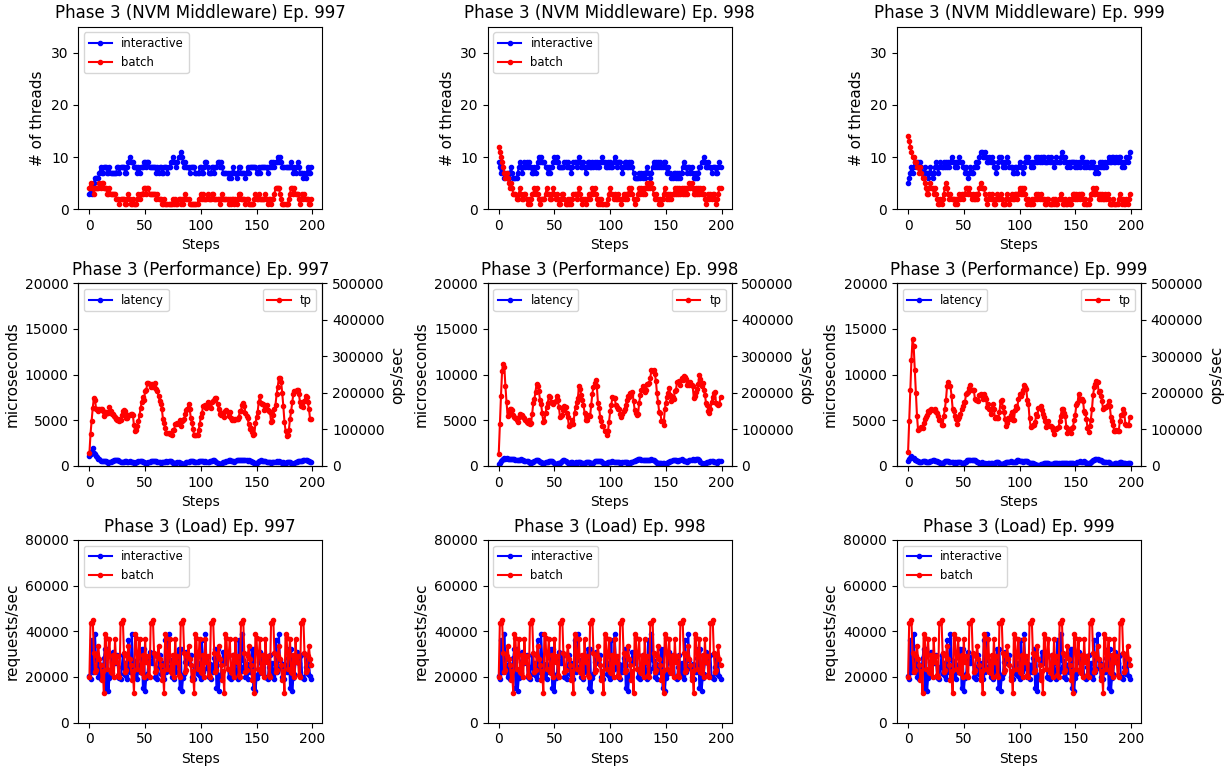
\includegraphics[width=\textwidth,height=\textheight,keepaspectratio,angle=0]{images/rl_training_phase3.png}
  % \caption{Learned Pattern Phase 3}
  \caption[Learned Pattern of Agent during Phase 3]{Visualization depicting the learned pattern of the agent during Phase 1 of the training process. The analysis focuses on the behavior observed in the final three episodes of the Q-Learning process, which spanned 1,000 episodes. During these episodes, the exploration rate is so low that the agent predominantly exploits its accumulated knowledge. The first row illustrates the agent's configuration of the NVM Middleware with approximately 8 interactive and low number of batch threads (approximately less than 5), aligning with preliminary results for Phase 3. In the middle row, the throughput and 99th percentile latency reported by the NVM Middleware at each time step are depicted. By employing the optimal combination of threads, the agent consistently maintains low latency (less than 250 microseconds) and a throughput exceeding 250,000 operations/second across most steps. Finally, the bottom row illustrates the operations per second sent to the NVM Middleware by Phase 3.}
  \label{fig:learned_phase_3}
\end{figure}

\begin{figure}[!htb]
  \centering
  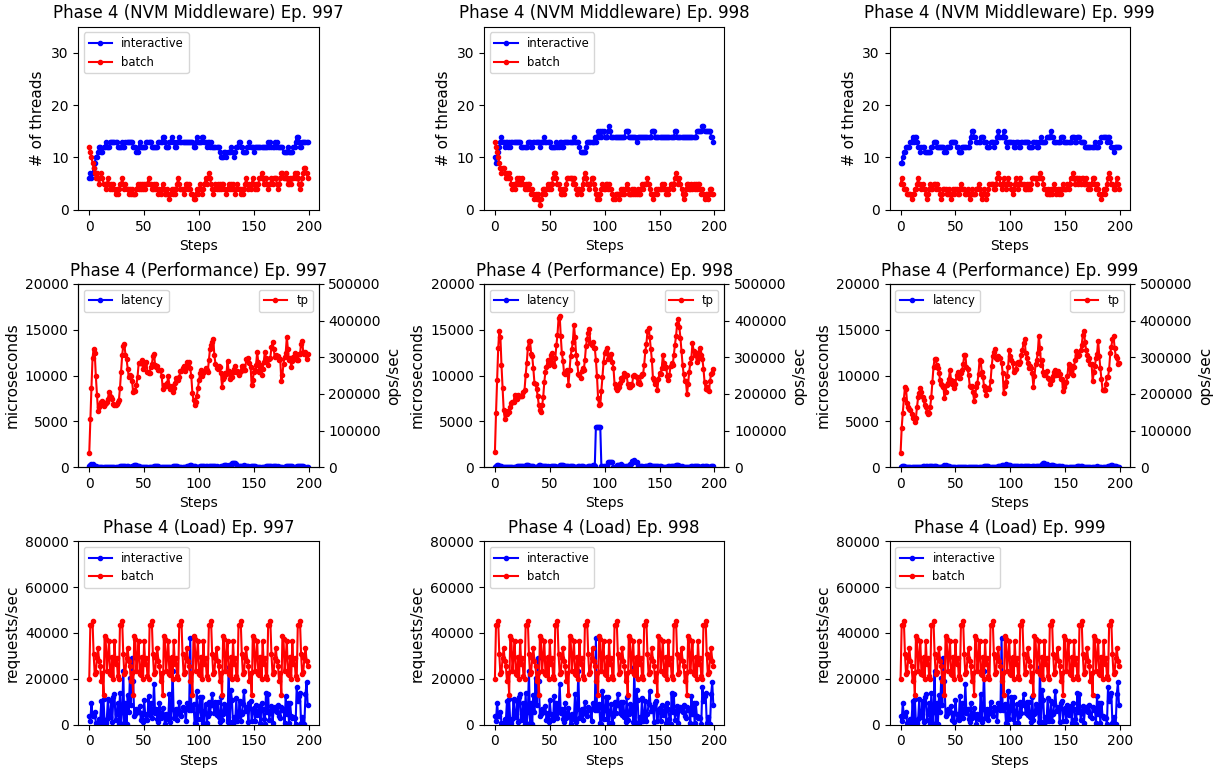
\includegraphics[width=\textwidth,height=\textheight,keepaspectratio,angle=0]{images/rl_training_phase4.png}
  % \caption{Learned Pattern Phase 4}
  \caption[Learned Pattern of Agent during Phase 3]{Visualization depicting the learned pattern of the agent during Phase 1 of the training process. The analysis focuses on the behavior observed in the final three episodes of the Q-Learning process, which spanned 1,000 episodes. During these episodes, the exploration rate is so low that the agent predominantly exploits its accumulated knowledge. The first row illustrates the agent's configuration of the NVM Middleware with high number of interactive threads (approximately 15) and low number of batch threads (approximately 5), aligning with preliminary results for Phase 4. In the middle row, the throughput and 99th percentile latency reported by the NVM Middleware at each time step are depicted. By employing the optimal combination of threads, the agent consistently maintains low latency (less than 250 microseconds) and a throughput exceeding 250,000 operations/second across most steps. Finally, the bottom row illustrates the operations per second sent to the NVM Middleware by Phase 4.}
  \label{fig:learned_phase_4}
\end{figure}

\FloatBarrier

\subsection*{Evaluating the RL Agent}

\begin{figure}[ht]
  \centering
  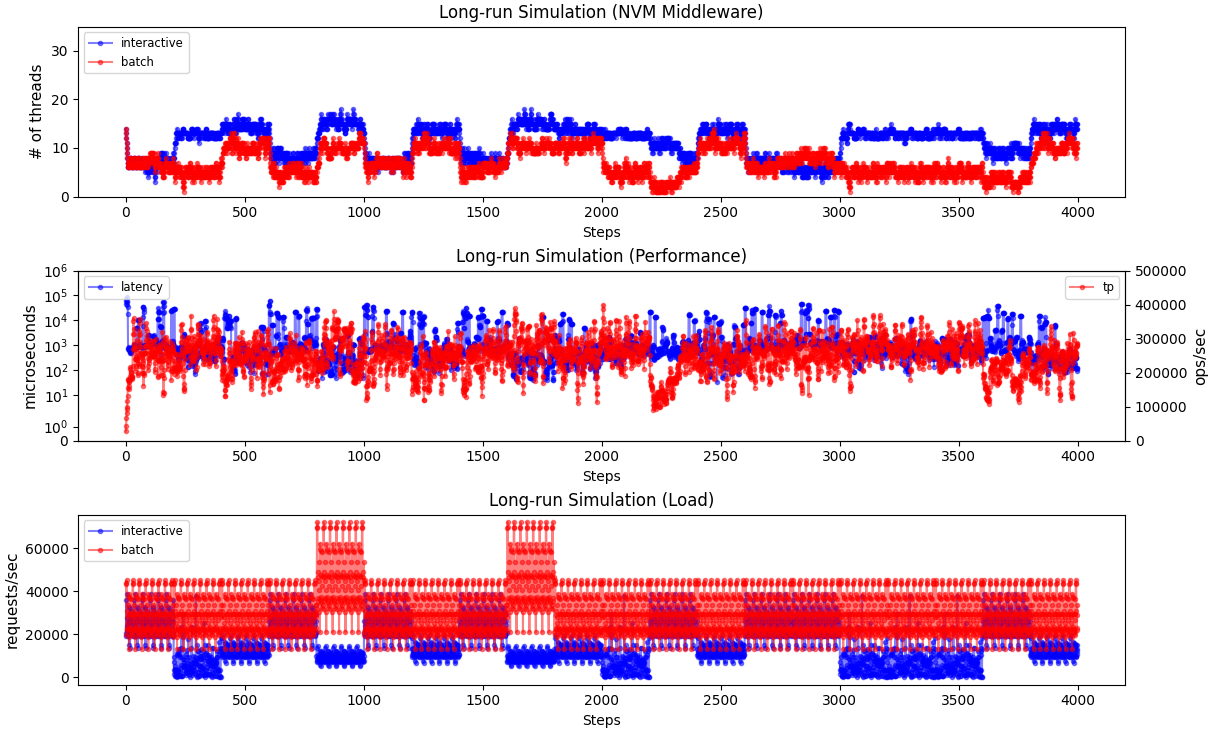
\includegraphics[width=\textwidth,height=\textheight,keepaspectratio]{images/long_run_sim.png}
  \caption[Reinforcement Learning Agent Adaptation to Shifting Workloads]{Illustration demonstrating the dynamic adjustment of thread counts by the RL agent during a test comprising 4,000 steps with randomly alternating phases. The top row showcases the RL agent's utilization of learned knowledge to optimize the number of interactive and batch threads for each phase. In the middle row, the throughput and 99th percentile latency reported by the NVM Middleware at each time step are depicted. By dynamically modifying the NVM Middleware threads, the throughput aligns with the predefined throughput SLA. However, unexpected spikes in the 99th percentile latency are observed, contrary to the training phase. The bottom row illustrates the operations per second sent by each phase, highlighting the shift in patterns every 200 steps.}
  \label{fig:long_run_eval}
\end{figure}

We evaluate the trained RL agent's performance against two baseline scenarios: one with disabled concurrency control in the NVM Middleware and another with a fixed policy of 15 interactive and batch threads. Each test comprises a long-run simulation spanning 4,000 steps, with the workload changing every 200 steps. We capture the minimum, 25th, 50th, 75th, and maximum throughput and tail latency observed by the NVM Middleware, as well as the environment rewards for each test. Figure \ref{fig:long_run_eval} illustrates the dynamic behavior of the RL agent as it adapts the combination of interactive and batch threads in response to the current workload patterns learned during training.

Our observations demonstrate the added performance benefits of RL-driven policies under varying workloads. While incorporating the NVM Middleware with a fixed policy yields performance improvements, dynamic control implemented by the RL agent further enhances performance. Increased rewards (Table \ref{table:eval_results_reward}) observed by the RL agent indicate superior maximization of performance and adherence to target SLAs. This is reflected in the achieved throughput (Table \ref{table:eval_results_tp}), with the NVM Middleware meeting the throughput target for 50\% of steps, compared to less than 25\% for the fixed policy scenario. Furthermore, although not achieving the target throughput in all steps, the NVM Middleware's overall throughput is closer to the target compared to the other scenarios.

However, in this experiment, the 99th percentile latency (Table \ref{table:eval_results_latency}) exhibited by both scenarios using the NVM Middleware did not meet expectations. We attribute this issue to the chosen interactive workloads not sufficiently stressing the system, leading to better performance in the scenario with no concurrency control. Further discussion on this topic is provided in Section 6.

\begin{table}[ht]
  \centering
  \caption[Reinforcement Learning Agent Reward Analysis in Long-run Test]{Analysis of the rewards achieved by the RL agent under shifting workloads compared to two baseline scenarios: one without concurrency control and the other keeping the NVM Middleware threads fixed. The values represent the distribution of reward signals reported by the environment at each time step, ranging from the minimum to the maximum observed, along with quartiles and median scores. Overall, the NVM Middleware with the RL agent achieves the highest reward.}
  \label{table:eval_results_reward}
  % Tabular environment goes AFTER the caption!
  % \begin{adjustbox}{width=1\textwidth}
  \begin{tabular}{|c|c|c|c|}
    % after \\: \hline or \cline{col1-col2} \cline{col3-col4} ...
    \hline
    \thead{} & \thead{No NVM Middleware} & \thead{NVM Middleware Fixed} & \thead{NVM Middleware + RL} \\
    \hline
    Min & -94,755.386 & -65,157.089 & \cellcolor{green}-87,907.434 \\\hline
    Q1 & -10,790.1 & -8,605.4625 & \cellcolor{green}-3,647.9454 \\\hline
    Median & -6,983.235 & -3,208.995 & \cellcolor{green}-4.005294 \\\hline
    Q3 & -4,042.9125 & -2.353015 & \cellcolor{green}0.31523 \\\hline
    Max & 3.174046 & 4.89667 & \cellcolor{green}4.582787 \\
    \hline
  \end{tabular}
% \end{adjustbox}
\end{table}

\begin{table}[ht]
  \centering
  \caption[Reinforcement Learning Agent Throughput Analysis in Long-run Test]{Analysis of the throughput achieved by the RL agent under shifting workloads compared to two baseline scenarios: one without concurrency control and the other keeping the NVM Middleware threads fixed. The values represent the distribution of throughput (operations/second) measurements reported by the NVM Middleware at each time step, ranging from the minimum to the maximum observed, along with quartiles and median scores. Overall, the NVM Middleware with the RL agent achieves the highest throughput.}
  \label{table:eval_results_tp}
  % Tabular environment goes AFTER the caption!
  % \begin{adjustbox}{width=1\textwidth}
  \begin{tabular}{|c|c|c|c|}
    % after \\: \hline or \cline{col1-col2} \cline{col3-col4} ...
    \hline
    \thead{} & \thead{No NVM Middleware} & \thead{NVM Middleware Fixed} & \thead{NVM Middleware + RL} \\
    \hline
    Min & 72,218.9 & 104,719.9 & \cellcolor{green}159,168.8 \\\hline
    Q1 & 112,440 & 148,792.5 & \cellcolor{green}218,816.25 \\\hline
    Median & 135,508.5 & 186,877 & \cellcolor{green}252,078.5 \\\hline
    Q3 & 166,340.25 & 231,597.75 & \cellcolor{green}278,205 \\\hline
    Max & 242,104.4 & 357,445.6 & \cellcolor{green}352,800.27 \\
    \hline
  \end{tabular}
% \end{adjustbox}
\end{table}

\begin{table}[ht]
  \centering
  \caption[Reinforcement Learning Agent Latency Analysis in Long-run Test]{Analysis of the throughput achieved by the RL agent under shifting workloads compared to two baseline scenarios: one without concurrency control and the other keeping the NVM Middleware threads fixed. The values represent the distribution of latency (microseconds) measurements reported by the NVM Middleware at each time step, ranging from the minimum to the maximum observed, along with quartiles and median scores. Surprisingly, in this particular test, both configurations involving the NVM Middleware exhibited higher latency compared to the baseline without concurrency control. This unexpected outcome suggests that the interactive workloads may not have adequately stressed the system, resulting in increased latency when utilizing the NVM Middleware. Further investigation is warranted to ascertain the underlying factors contributing to this behavior.}
  \label{table:eval_results_latency}
  % Tabular environment goes AFTER the caption!
  % \begin{adjustbox}{width=1\textwidth}
  \begin{tabular}{|c|c|c|c|}
    % after \\: \hline or \cline{col1-col2} \cline{col3-col4} ...
    \hline
    \thead{} & \thead{No NVM Middleware} & \thead{NVM Middleware Fixed} & \thead{NVM Middleware + RL} \\
    \hline
    Min & \cellcolor{green}19 & 89 & 130.95 \\\hline
    Q1 & \cellcolor{green}81 & 239 & 396.75 \\\hline
    Median & \cellcolor{green}19 & 674.5 & 754 \\\hline
    Q3 & \cellcolor{green}271.5 & 1,888.75 & 1,427 \\\hline
    Max & \cellcolor{green}82,824 & 34,090.93 & 34,712.04 \\
    \hline
  \end{tabular}
% \end{adjustbox}
\end{table}
